\documentclass[12pt]{article}
\usepackage{graphicx}
\usepackage[utf8]{inputenc}
\usepackage[czech]{babel}
\usepackage{czech}
\usepackage[tables,figures]{updiplom}
\usepackage{url}
\DeclareUrlCommand\url{\def\UrlLeft{<}\def\UrlRight{>} \urlstyle{tt}}
\usepackage{amssymb}
\usepackage{graphicx}
\usepackage{ae}


\title{Kryptoanalýza historických šifer}
%\subtitle{Cryptanalysis historical ciphers}
\author{Lukáš Havrlant}
\year{2010}
\date{25. květen}

\annotation{%
%Luštění šifer bylo v historii náročné na čase i na lidské zdroje. Dnes můžeme luštění historických šifer automatizovat pomocí počítače. V této práci se budu zabývat návrhem a realizací algoritmů, které dokáží v řádu sekund automaticky rozluštit šifrové texty zašifrované vybranými historickými šiframi.  
Automatizované luštění šifer počítačem dnes může plně nahradit těžkou a zdlouhavou práci historických kryptoanalytiků. V~práci se zabývám návrhem a realizací algoritmů, které dokáží v~řádu sekund automaticky rozluštit zprávu zašifrovanou některou z~vybraných historických šifer.
}

\thanks{%
Děkuji RNDr. Miroslavu Kolaříkovi, Ph.D. za vedení této bakalářské práce a za rady při konzultacích.}

\newcounter{proofcounter}
\setcounter{proofcounter}{0}

\theoremstyle{definition}
\newtheorem{crypto}{Kryptosystém}

%%% Definice příkazů
\newcommand{\var}[1]{\texttt{#1}}
\newcommand{\code}[1]{\texttt{#1}}
\newcommand{\stats}{\xi}
\newcommand{\ovl}[1]{(ovládací prvek \ref{#1})}
\newcommand{\cit}[1]{--- Citováno z~\cite{#1}.}



\newcommand{\setp}{\mathcal{P}}
\newcommand{\setc}{\mathcal{C}}
\newcommand{\setk}{\mathcal{K}}
\newcommand{\setd}{\mathcal{D}}
\newcommand{\sete}{\mathcal{E}}
\newcommand{\setz}{\mathbb{Z}}

\renewcommand{\mod}{\mbox{mod\,}}
\newcommand{\alp}{_{26}}


\clubpenalty 10000
\widowpenalty 10000


\begin{document}

\hyphenation{nej-mo-der-něj-ší}
\hyphenation{opo-zi-ce}
\hyphenation{ope-ra-ce-mi}
\hyphenation{ta-bul-ka}
\hyphenation{zdlou-ha-vou}
\hyphenation{zá-kla-dě}
\hyphenation{nej-mé-ně}


\maketitle
\newpage

\section{Slovníček pojmů}

V~tomto textu se zabývám výhradně historickými šiframi. Některé definice tak byly upraveny na úkor obecnosti, aby lépe popisovaly vztah k~těmto šifrám. 

\subsection{Kryptologie}
Kryptologie je věda zabývající se obecně šifrováním. 

\subsection{Kryptografie}
Kryptografie je podobor kryptologie a zabývá se návrhem a realizací šifrovacích algoritmů.

\subsection{Kryptoanalýza}
Kryptoanalýza je podobor kryptologie a zabývá se prolamováním a luštěním šifrovacích algoritmů. 

\subsection{Otevřený text}
Otevřený text je libovolný text, který chce uživatel zašifrovat. Obyčejně se jedná o~nějakou zprávu v~běžném jazyce, která by se neměla dostat do rukou každému, ale typicky pouze vybrané skupině jiných uživatelů. V~této práci bude otevřený text vždy psán malými písmeny.

\subsection{Šifrový text}
Šifrový text je takový text, který v~sobě ukrývá původní otevřený text, ale čtenář není schopný tento otevřený text z~šifrového textu bez dalších dodatečných informací získat. Šifrový text může čtenáři připadat jako náhodná posloupnost znaků. V~této práci bude šifrový text vždy psán velkými písmeny.

\subsection{Šifrovací klíč}
Šifrovací klíč je libovolná posloupnost písmen (často reálná slova), která spolu s~použitou šifrou specifikuje, jakým způsobem se má otevřený text proměnit na šifrový text a naopak -- jak z~šifrového textu dostat zpět otevřený text. 

Většina šifer obsahuje i klíče, které jsou sice platným vstupem do algoritmu, nicméně výsledný šifrový text je buď identický s~otevřeným textem nebo je text velice podobný a na první pohled odhalitelný. Takové klíče se nazývají {\em slabé klíče}. 

\subsection{Šifra, šifrování}
Šifra je algoritmus, který bere na vstupu otevřený text a šifrovací klíč a na výstupu vrátí šifrový text. Cílem šifry pak je vytvořit zašifrovanou zprávu, kterou bude schopný přečíst každý, komu je zpráva určena, ale nikdo nepovolaný. V~praxi to znamená, že příjemce zašifrované zprávy musí znát jednak použitou šifru a dále použitý šifrovací klíč, aby byl schopen si přečíst původní otevřený text. Pro všechny ostatní by mělo být nemožné bez těchto informací otevřený text získat. 

Přestože příjemce potřebuje znát jak použitou šifru, tak použitý klíč, obyčejně se nestaví zabezpečení zprávy na neznalosti použité šifry, ale hlavně na neznalosti klíče. I~pokud zná útočník veškeré detaily o~šifře, neměl by být schopný rozluštit ze šifrového textu původní otevřený text, pokud nezná klíč.

Poznámka: Šifrování má blízko ke steganografii, což je věda zabývající se skrytím komunikace tak, aby si ostatní pozorovatelé ani nevšimli, že vůbec nějaká komunikace probíhá. Zpozorování komunikace se rovná prolomení steganografie. Naopak zašifrovanou zprávu můžeme poslat i nezabezpečenými veřejnými cestami, bezpečnost dat je zajištěna utajením klíče. 

Opačný proces k~šifrování je dešifrování. 

V~praxi existují dvě základní techniky šifrování: substituční a transpoziční.

\subsubsection{Substituční šifra}
Substituční šifra provádí záměny částí textu za jiné části textu podle nějakého klíče. Časté jsou například záměny jednotlivých písmen za jiná písmena, místo \uv{a} můžeme v~šifrovém textu napsat \uv{b}. Při dešifrování pak obvykle provádíme opačný postup, místo \uv{b} píšeme \uv{a}. 

Dále můžeme rozlišovat, s~kolika šifrovými abecedami šifra pracuje. Při použití jedné abecedy platí, že každé písmeno má pouze jednu substituci. Pokud použijeme více abeced, má každé písmeno více možných substitucí, přičemž kterou substituci zrovna použijeme rozhoduje šifrovací klíč. Šifra která používá jednu abecedu se nazývá {\em monoalfabetická}; šifra která používá více abeced se nazývá {\em polyalfabetická}. 

\subsubsection{Transpoziční šifra}
Transpoziční šifra mění pořadí znaků v~otevřeném textu. V~šifrovém textu zůstávají všechna písmena, která jsou i v~otevřeném textu, ale jsou zpřeházena podle nějakého klíče. Primitivní transpoziční šifrou pak může být například napsání textu pozpátku. 

\subsubsection{Kombinované šifry}

Další typy šifer zpravidla vznikají kombinací těchto dvou typů šifer. I~nejmodernější šifry jako DES či AES jsou založeny na složitých kombinací transpozic a substitucí.

\subsection{Alice, Bob a Eva}
Alice a Bob jsou dva lidé, uživatelé, kteří si chtějí navzájem poslat zprávu a typicky nechtějí, aby si obsah zprávy mohl přečíst někdo jiný. Alice posílá zprávu Bobovi. Eva je potenciální útočník, který se může dostat ke zprávě, přečíst si ji a případně ji rozluštit. Eva je pouze pasivní útočník, nemůže měnit obsah zprávy. 

\subsection{Obraz a vzor písmene}
V~substitučních šifrách je obraz písmene takové písmeno, na které se zobrazí písmeno z~otevřeného textu. Pokud platí substituce a$\rightarrow$b, písmeno \uv{b} je obrazem písmene \uv{a}. Naopak písmeno \uv{a} je vzorem písmene \uv{b}. Podobně můžeme definovat i obraz respektive vzor slova atp. 

\subsection{Abeceda}
Pod pojmem abeceda budeme rozumět standardní anglickou abecedu a-zA-Z. Přestože je teoreticky i technicky možné, abychom při šifrování používali národní abecedy, obyčejně bývá zvykem používat právě anglickou abecedu. Algoritmy popsané v~této práci jsou nicméně obecné a zvládly by bez dalších úprav přechod na národní abecedu. 



\newpage
\section{Popis šifer}





\subsection{Základní definice}
\label{defs}
\subsubsection{Kryptosystém}
Kryptosystém je pětice $(\setp, \setc, \setk, \sete, \setd)$, která splňuje následující podmínky:

\begin{enumerate}
\item $\setp$ je konečná množina všech možných otevřených textů;
\item $\setc$ je konečná množina všech možných šifrových textů;
\item $\setk$ je konečná množina všech možných šifrovacích klíčů;
\item Pro každé $K\in \setk$ existuje šifrovací pravidlo $e_K\in\sete$ a odpovídající dešifrovací pravidlo $d_K\in\setd$. Všechna $e_K:\setp\rightarrow\setc$ a $d_K:\setc\rightarrow\setp$ jsou zobrazení, pro která platí $d_K\left(e_K\left(x\right)\right)=x$ pro každý otevřený text $x\in\setp$.
\end{enumerate}

Nejdůležitější bod je čtvrtý -- říká nám, že pokud zašifrujeme text pomocí nějakého klíče, pak při dešifrování šifrového textu se stejným klíčem získáme původní otevřený text. 



\subsubsection{Proces šifrování}
Na začátku si musí Alice s~Bobem nějakým bezpečným kanálem předat klíč $K\in\setk$. Následně chce Alice poslat šifrovanou zprávu Bobovi. Tato zpráva už nemusí jít bezpečným kanálem. Předpokládáme, že zpráva je řetězec ve tvaru: 

$$x=x_1x_2\ldots x_n,$$
kde $n\in\mathbb{N} \wedge n\ge1$ a $x_i\in\setp, 1\le i \le n$. Každé $x_i$ je pak zašifrováno pomocí $e_K$. Alice spočítá
 $$y_i=e_K\left(x_i\right), 1\le i \le n.$$  
Výsledný šifrový text $y$ Alice získá zřetězením dílčích výsledků:
$$y=y_1y_2\ldots y_n.$$
Tento řetězec je poslán nezabezpečeným kanálem. Když Bob přijme zprávu, dešifruje ji: 

$$x_i=d_K\left(y_i\right), 1\le i \le n$$
a původní otevřenou zprávu získá zřetězením:

$$x=x_1x_2\ldots x_n.$$

Zobrazení $e_K$ musí být zřejmě injektivní, má-li být šifrování jednoznačné. Pokud by totiž platilo

$$y=e_K(x_1)=e_K(x_2),$$
kde $x_1\ne x_2$, nebylo by jasné, kterou z~těchto dvou zpráv Alice Bobovi poslala. Celý proces šifrování znázorňuje diagram na obrázku \ref{img_cryptosystem}

\begin{figure}[h]
  \begin{center}
  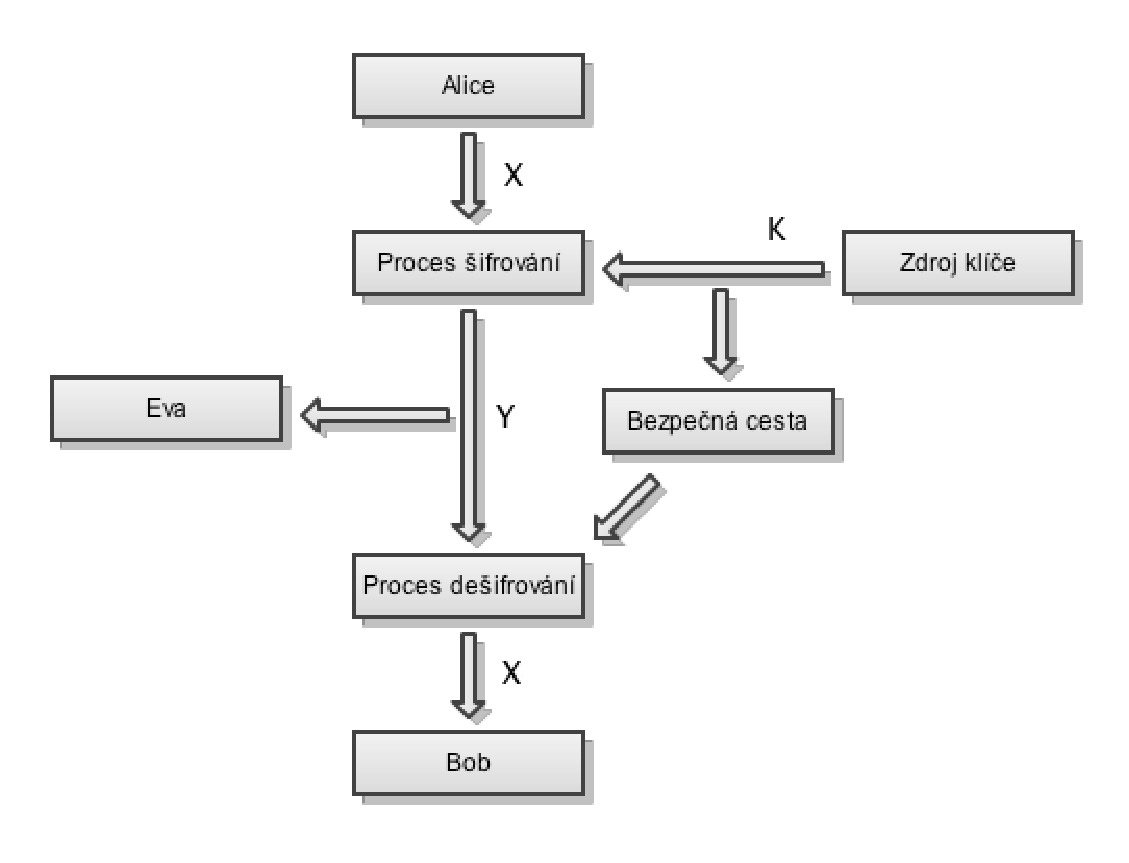
\includegraphics[scale=0.8]{images/cryptosystem.eps}
  \end{center}
\caption{Komunikace šifrovým kanálem}
\label{img_cryptosystem}
\end{figure}

\subsubsection{Modulární aritmetika}
Nechť $a, b\in\mathbb{N}_0$ a $m\in\mathbb{N}$. Pak píšeme

$$a\equiv b \,(\mod m),$$
pokud $m$ dělí $b-a$. Čteme \uv{$a$ je kongruentní s~$b$ modulo $m$}. Notaci bez závorek $a\, \mod m$ budeme používat k~označení zbytku po celočíselném dělení, tj. pokud v~tomto případě platí $a=x\cdot m+r\wedge r < m; x,r\in\mathbb{N}_0$, pak $a\,\mod b = r$.

Definujme okruh $\setz_m$: $\setz_m$ je množina $\left\{0, 1, \ldots, m-1\right\}$ s~definovanými operacemi sčítání $+$ a násobení $\times$. Tyto operace fungují stejně jako běžné operace sčítání a násobení, pouze s~tím rozdílem, že výsledek je redukován modulo $m$. Máme-li čísla $a,b\in\mathbb{N}_0$ a $a_m,b_m\in \setz_m$ taková, že $a=a_m\wedge b=b_m$, pak platí:

$$a_m+b_m=(a+b)\, \mod m$$
a stejně tak:

$$a_m\times b_m=(a\cdot b)\, \mod m.$$

Příklad: Pokud bychom měli okruh $\setz_{10}$ a chtěli vypočítat $7\times9$, vypočítáme nejprve $7\cdot9=63$ a následně provedeme modulo: $63\,\mod 10 = 3$. Výsledek je tři. 

Protože $\setz_m$ je okruh, musí pro každé číslo $x_m\in\setz_m$ existovat i inverzní číslo $x'_m\in\setz_m$, pro které platí $x_m+x'_m=0$. Protože se nepohybujeme v~záporných číslech, nemůžeme k~číslu $x$ přičíst jeho záporný ekvivalent, ale můžeme využít modularity a přičíst k~$x_m$ takové číslo $x'_m$, které dá v~součtu číslo $m$, protože platí $m\,\mod m=0$. Inverzní prvek $x'_m\in\setz_m$ k~prvku $x_m\in\setz_m$ můžeme definovat jako

$$x' = m-x,$$
kde $x,x'\in\mathbb{N}_0$ a zároveň $x = x_m\, \wedge\, x'=x'_m$. Tímto způsobem můžeme realizovat odečítání v~$\setz_m$:

$$(a_m-b_m)\,\mod m = (a_m+b'_m)\,\mod m.$$

Přestože následující šifry pracují výhradně s~písmeny anglické abecedy, budeme v~definicích používat pouze čísla. Převod čísel na písmena a naopak realizujeme jednoduchou substitucí $a\leftrightarrow 0, b\leftrightarrow 1, c\leftrightarrow 2, \ldots, z\leftrightarrow 25$. 


Definice zavedené v~kapitole \ref{defs} pochází z~knihy \cite{cryptography}.


%%%%%%%%%%%%%%%%%%%%%%%%%%%%%%%%%%%%%%%%%%%%%%%%%%%%%%%%%%%%%%%%
%%%%%%%%%%%%%%%%%%%%%%%%% CAESAROVA ŠIFRA %%%%%%%%%%%%%%%%%%%%%%%%%
%%%%%%%%%%%%%%%%%%%%%%%%%%%%%%%%%%%%%%%%%%%%%%%%%%%%%%%%%%%%%%%%


\subsection{Caesarova šifra}
\label{caesar}
\subsubsection{Definice}
\begin{crypto}

Nechť $\setp=\setc=\setk=\setz\alp$. Pro $0\le K \le 25$ a $x,y\in\setz\alp$ definujeme

$$e_K\left(x\right)=\left(x+K\right)\,\mod 26$$
a

$$d_K\left(y\right)=\left(y-K\right)\,\mod 26.$$
\end{crypto}

\cit{cryptography}

\subsubsection{Historie}
Caesarova šifra je jednoduchá substituční šifra pojmenována po římském vojevůdci Juliu Caesarovi, který tuto šifru používal. Jedná se o~vůbec první dokumentovaný záznam použití substituční šifry pro vojenské účely. Zmínka o~ní se nachází v~publikaci {\em Zápisky o~válce galské}, ve které Caesar popisuje, jak poslal zprávu Ciceronovi, který byl obklíčen nepřítelem: 

\begin{quotation} 
\uv{\em Posel dostal rozkaz, ať vhodí kopí s~připevněnou zprávou přes hradby tábora, pokud by se nemohl dostat dovnitř. Tak se i stalo. Gal, vystrašený možným nebezpečím, mrštil kopí. Nešťastnou náhodou se stalo, že se kopí zabodlo do věže. Teprve třetího dne si ho povšiml jeden z~vojáků, který kopí sejmul a zanesl Ciceronovi. Ten si přečetl zprávu a poté ji oznámil svým vojákům, což všem přineslo velikou radost.}
\end{quotation}

\cit{singh}

\subsubsection{Popis šifry}
Caesarova šifra je speciálním případem monoalfabetické substituční šifry, viz kapitola \ref{mono} Na začátku šifrování si zvolíme klíč, který nám bude říkat, o~kolik písmen posuneme každé písmeno v~otevřeném textu. Tento klíč bude reprezentován jedním písmenem abecedy, přičemž platí, že písmeno \uv{a} značí posun o~nula písmen, písmeno \uv{b} o~jedno písmeno atd. Výsledný šifrový text získáme tak, že každé písmeno v~otevřeném textu posuneme o~tolik písmen dál, kolik určuje klíč. Máme-li posunovat o~tři písmena (klíčem je písmeno \uv{d}), tak pokud máme v~otevřeném textu písmeno \uv{a}, v~šifrovém textu bude písmeno \uv{D}, dále pak b$\rightarrow$E, c$\rightarrow$F, \dots Přehledně to zobrazuje následující tabulka, v~prvním řádku je otevřená abeceda, ve druhém šifrová:

\begin{verbatim}
                     abcdefghijklmnopqrstuvwxyz
                     DEFGHIJKLMNOPQRSTUVWXYZABC
\end{verbatim}

Jak je vidět, klíč zároveň udává, na které písmeno se v~šifrovém textu zobrazí písmeno \uv{a}. 

Příklad: text \uv{prsi a venku se setmelo} by s~klíčem \uv{k} dal při použití Caesarovy šifry výsledek \uv{ZBCS K~FOXUE CO CODWOVY}. 

\subsubsection{Výhody}

\begin{itemize}
\item Šifra je především jednoduchá a rychlá. Zašifrovat text Caesarovou šifrou zvládne každý i bez jakékoliv dodatečné pomůcky. 
\end{itemize}

\subsubsection{Nevýhody}
\begin{itemize}
\item Šifra obsahuje pouze velmi omezené množství klíčů. Anglická abeceda obsahuje 26 písmen, které můžeme použít jako klíč. Nicméně pokud použijeme jako klíč písmeno \uv{a}, šifrový text se nijak nezmění, jedná se o~slabý klíč. V~úvahu připadá pouze 25 písmen, které můžeme použít jako šifrovací klíč. Takové množství klíčů je velmi malé a potenciální útočník je schopen ručně vyzkoušet všechny klíče v~řádu minut. 
\item Výsledný šifrový text si uchovává informace o~četnosti písmen v~otevřeném textu. Pokud se například v~otevřeném textu vyskytlo písmeno \uv{e} celkem stokrát, v~šifrovém textu musí být nějaké písmeno, které se tam také vyskytuje stokrát. 
\item Šifrový text zachovává vzdálenosti mezi písmeny. Pokud jsou v~otevřené abecedě písmena \uv{a} a \uv{e} od sebe vzdálena o~čtyři písmena, budou jejich obrazy v~šifrové abecedě také vzdáleny o~čtyři písmena.
\end{itemize}

Zdroje ke kapitole \ref{caesar}: \cite{vondruska} a \cite{singh}.










%%%%%%%%%%%%%%%%%%%%%%%%%%%%%%%%%%%%%%%%%%%%%%%%%%%%%%%%%%%%%%%%%%%%%
%%%%%%%%%%%%%%%%%%%%%%%%% MONOALFABETICKÁ ŠIFRA %%%%%%%%%%%%%%%%%%%%%%%%%
%%%%%%%%%%%%%%%%%%%%%%%%%%%%%%%%%%%%%%%%%%%%%%%%%%%%%%%%%%%%%%%%%%%%%


\subsection{Monoalfabetická substituční šifra}
\label{mono} 
\subsubsection{Definice}
\begin{crypto}
Nechť $\setp=\setc=\setz\alp$. Množina $\setk$ obsahuje všechny permutace skupiny 26 symbolů $0,1,2\ldots,25$. Pro každou permutaci $\pi\in\setk$ definujme 

$$e_\pi\left(x\right)=\pi(x),$$
a 

$$d_\pi\left(y\right)=\pi^{-1}\left(y\right),$$
kde $\pi^{-1}$ je inverzní permutace k~$\pi$. 
\end{crypto}

\cit{cryptography}

\subsubsection{Popis šifry}
Tato šifra funguje podobně jako Caesarova šifra, pouze nemá nijak omezené možné substituce. Na začátku si musíme vytvořit tabulku substitucí, která nám bude určovat, na co se mají jednotlivá písmena z~otevřeného textu zobrazit. Zobrazení musí být jednoznačné, aby bylo následně jednoznačné i dešifrování. Tabulka substitucí může vypadat například takto:

\begin{verbatim}
                     abcdefghijklmnopqrstuvwxyz
                     MUNBQPEKVZAJTXRCWSYLGIFDOH
\end{verbatim}

V~první řadě je opět otevřená abeceda, ve druhé řadě šifrová abeceda. Ta je poskládána náhodně (respektive jak zrovna chceme), není třeba dodržovat pravidlo posunutí jako u~Caesarovy šifry. Výsledný šifrový text vznikne záměnou písmen z~otevřené abecedy za jejich obrazy v~šifrové abecedě. V~tomto případě bychom místo písmene \uv{a} napsali písmeno \uv{M}, dále b$\rightarrow$U, c$\rightarrow$N,~\dots Dešifrování by probíhalo stejně, pouze s~obrácenou tabulkou substitucí, tj. N$\rightarrow$c,~\dots

Příklad: text \uv{tato noc nebude kratka} by s~klíčem \uv{munbqpekvzajtxrcwsylgifdoh} dal při použití monoalfabetické šifry výsledek \uv{LMLR XRN XQUGBQ ASMLAM}. 

Aby si uživatel nemusel pamatovat celou přeházenou abecedu, je možné zvolit si heslo, pomocí něhož se vygeneruje požadovaný klíč. Heslem může být libovolné slovo nebo věta, klíč se poté vygeneruje tak, že se z~hesla odstraní všechny vícenásobné výskyty písmen -- nechá se pouze první výskyt písmene -- a doplní se chybějící písmena v~abecedním pořadí. Pokud máme heslo \uv{informatika}, po odstranění zdvojených písmen dostáváme \uv{informatk} a po doplnění písmen získáme klíč \uv{informatkbcdeghjlpqsuwxyz}. 

\subsubsection{Výhody}

\begin{itemize}
\item Šifra je jednoduchá, její použití není o~moc složitější než u~Caesarovy šifry. Po vytvoření tabulky substitucí je použití prakticky stejné.
\item Velký počet klíčů. Největší slabinou Caesarovy šifry byl nízký počet klíčů (26), monoalfabetická substituční šifra používá jako klíč všechny permutace anglické abecedy, existuje tedy celkem $26!$ možných klíčů, což je přibližně $4\cdot10^{26}$ klíčů. Pokud by hypotetický počítač byl schopen ověřit miliardu klíčů za sekundu, trvalo by celkem dvanáct miliard let, než by prověřil všechny možné klíče. Jestli by tento počítač testoval pro každou zašifrovanou zprávu všech $26!$ klíčů, tak začal by-li s~testováním okamžitě při vzniku vesmíru, luštil by dnes teprve druhou zašifrovanou zprávu. Některé z~těchto klíčů jsou ovšem slabé klíče -- to jsou takové klíče, které mají mnoho substitucí ve tvaru x$\rightarrow$x. I~po odstranění těchto klíčů zůstává množina možných klíčů dostatečně velká. 
\item Na rozdíl od Caesarovy šifry nemusí být šifrová abeceda jen posunutá otevřená abeceda, takže šifra netrpí nevýhodou v~podobě stejné vzdálenosti písmen. 
\end{itemize}

%antisux
\newpage
\subsubsection{Nevýhody}

\begin{itemize}
\item Stejně jako u~Caesarovy šifry si šifrový text s~sebou nese informace o~frekvenci jednotlivých písmen. Při útoku můžeme využít klasickou frekvenční analýzu, ve které budeme zkoumat procentuální výskyt jednotlivých znaků, bigramů, trigramů apod. Pokud text obsahuje mezery a jsou tak zřejmá jednotlivá zašifrovaná slova, můžeme též využít frekvence písmen na začátku a na konci slov. Můžeme využít i další vztahy daného jazyka, například v~češtině se často za souhláskami vyskytuje méně různých písmen než za samohláskami. 
\item Obsahuje-li šifrový text mezery, můžeme zkusit najít taková slova, která mají i po zašifrování stejný {\em kanonický tvar}, viz kapitola \ref{kanon} I~po zašifrování si totiž slovo uchovává informace o~vztazích mezi obsaženými písmeny. Slovo v~otevřeném textu, které začíná i končí na stejné písmeno, bude začínat a končit na stejné písmeno i v~zašifrovaném textu. A~podobně pro všechny dvojice písmen ve slově. Pokud máme k~dispozici slovník daného jazyka, můžeme nalézt taková {\em unikátní slova}, která mají v~rámci slovníku zcela unikátní kanonický tvar. Pokud pak tento tvar nalezneme i v~šifrovém textu, bude to pravděpodobně ono {\em unikátní slovo}. Tento postup lze v~omezené míře aplikovat i pokud neznáme hranice mezi slovy. 
\end{itemize}

\subsubsection{Jak zvýšit bezpečnost šifry}
Šifru lze některými úpravami otevřeného textu vylepšit bez zásadních úprav šifrového algoritmu:

\begin{itemize}
\item Obě popsané nevýhody staví na tom, že text bude vykazovat známky běžného textu daného jazyka. Pokud upravíme otevřený text tak, že se nebude tvářit jako běžný text, ztížíme použití kryptoanalytických metod. Úpravy ovšem musí být takového charakteru, aby příjemce zprávy byl stále schopen text přečíst. V~úvahu tak připadají různé \uv{gramatycké chibi a přkleepi}, které útočníkovi ztíží práci, ale příjemce text pochopí. 
\item Účinné vylepšení je používání {\em nomenklátorů}, což jsou zástupné symboly pro určitá slova. Bob s~Alicí se mohou domluvit na tom, že určitá specifická a důležitá slova nahradí speciálním symbolem nebo obrázkem. Například \uv{kostel} bude obrázek kytary a \uv{továrna} obrázek nosorožce. Otevřený text \uv{Mrtvolu zakopeme za továrnou.} by se šifroval tak, že část \uv{Mrtvolu zakopeme za} by se zašifrovala monoalfabetickou šifrou podle zvoleného klíče a na místo továrny by se nakreslil obrázek nosorožce. I~pokud by Eva zjistila šifrový klíč, stejně by nevěděla, kam chtějí Bob s~Alicí mrtvolu zakopat. 
\item Při šifrování může Alice vložit do textu klamače neboli nuly. To jsou takové symboly, které nemají žádný význam, Bob ví, že nemají žádný význam, ale útočníka zmatou, protože se jeví jako reálné písmeno. Bob při dešifrování zprávy klamače automaticky zahazuje, ale Eva musí nejprve nějakým způsobem zjistit, které symboly jsou klamače a které symboly jsou reálná (zašifrovaná) písmena. Toto vylepšení je velmi efektivní, ale čím více klamačů zpráva obsahuje, tím více narůstá její velikost.
\end{itemize}

Zdroje ke kapitole \ref{mono}: \cite{chip}, \cite{singh} a \cite{mono}.







%%%%%%%%%%%%%%%%%%%%%%%%%%%%%%%%%%%%%%%%%%%%%%%%%%%%%%%%%%%%%%%%
%%%%%%%%%%%%%%%%%%%%%%%%% VIGENEROVA ŠIFRA %%%%%%%%%%%%%%%%%%%%%%%%%
%%%%%%%%%%%%%%%%%%%%%%%%%%%%%%%%%%%%%%%%%%%%%%%%%%%%%%%%%%%%%%%%




\subsection{Vigenèrova šifra}
\label{vigcipher}
\subsubsection{Definice}
\begin{crypto}
Nechť $\setp=\setc=\setk=\left(\setz\alp\right)^m$. Pro klíč $K=\left(k_1,k_2,\ldots,k_m\right)\in\setk$ definujme

$$e_K\left(x_1,x_2,\ldots,x_m\right) = \left(x_1+k_1,x_2+k_2,\ldots,x_m+k_m\right)$$
a

$$d_K\left(y_1,y_2,\ldots,y_m\right)=\left(y_1-k_1, y_2-k_2,\ldots,y_m-k_m\right),$$
kde jsou všechny operace prováděny v~$\setz\alp$.
\end{crypto}

\cit{cryptography}

\subsubsection{Historie}
Roku 1587 nechala královna Alžběta pro údajnou podporu katolické opozice popravit Marii Stuartovnu. K~tomuto činu přispělo i to, že Marie Stuartovna používala pro svou korespondenci mírně vylepšenou monoalfabetickou šifru, kterou bohužel pro Marii královnini luštiči prolomili a rozluštěná šifra sloužila jako jeden z~usvědčujících důkazů. Bylo jasné, že kryptografové musí vymyslet novou, silnější šifru, protože monoalfabetická substituční již nestačila.

Základní koncept Vigenèrovy šifry vymyslel v~60. letech 15. století florentský polyhistor Leon Battista Alberti, který jako první objevil a sepsal myšlenku polyalfabetické šifry -- šifry, která využívá více než jednu šifrovou abecedu. Konečnou podobu ale vymyslel francouzský diplomat Blaise de Vigenère. Ve své době se šifře přezdívalo {\em Le chiffre indèchiffrable} (česky: nerozluštitelná šifra). 

\subsubsection{Popis šifry}
Vigenèrova šifra je polyalfabetická substituční šifra, která používá až 26 šifrových abeced. Klíč tvoří libovolně dlouhé slovo, nicméně klíč by neměl obsahovat pouze jedno písmeno, protože by se pak šifra degradovala na Caesarovu šifru. Při šifrování se dále používá Vigenèrův čtverec, což je složitější tabulka substitucí, viz obrázek \ref{img_recta}

\begin{figure}[h]
  \begin{center}
  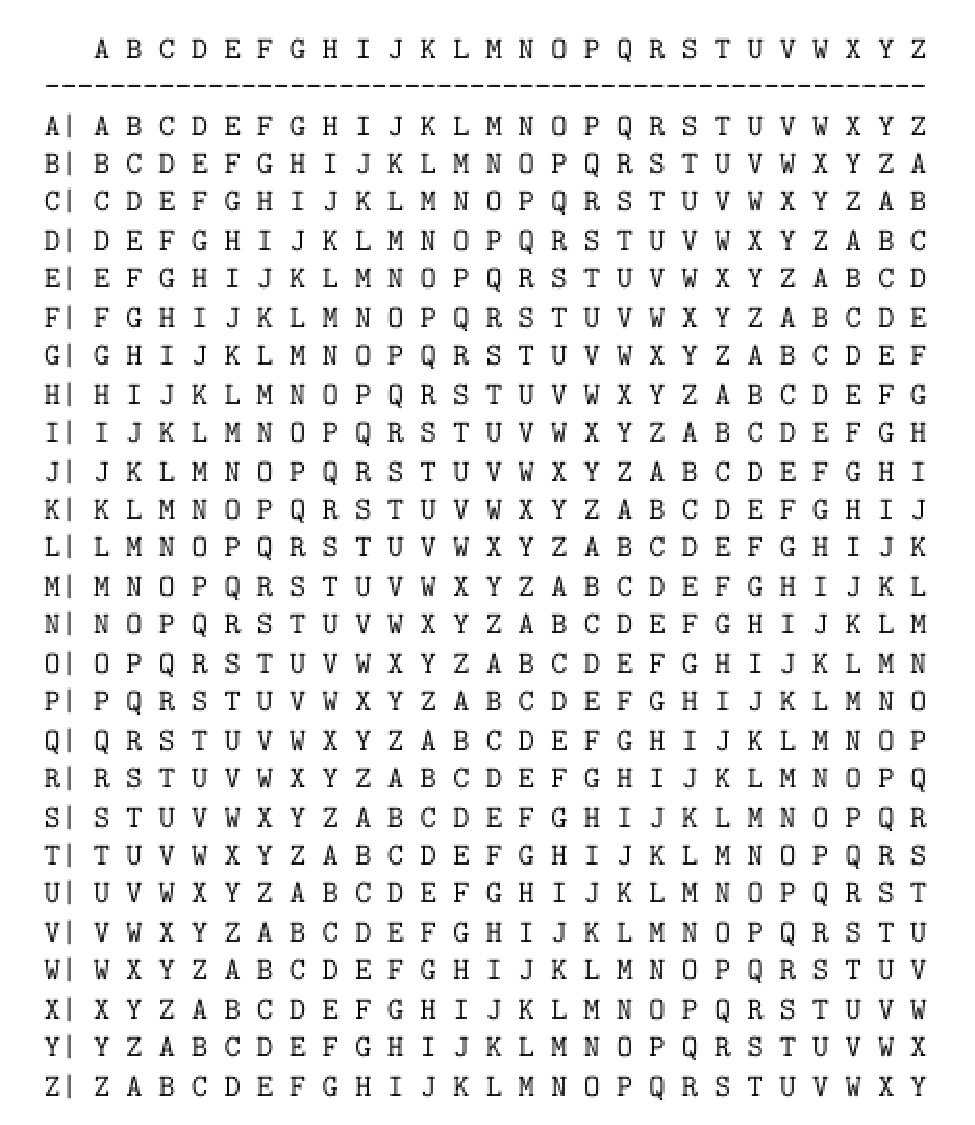
\includegraphics[scale=0.75]{images/recta.eps}
  \end{center}
\caption{Vigenèrův čtverec}
\label{img_recta}
\end{figure}

Na každém řádku se nachází jedna šifrová abeceda. Kterou šifrovou abecedu zrovna použijeme určuje klíč. V~prvním řádku budeme hledat písmena otevřeného textu a v~prvním sloupci písmena klíče. Výsledné písmeno šifrové abecedy nalezneme v~průsečíku tohoto řádku a sloupce. V~otevřeném textu postupujeme jednoduše stále kupředu po jednom písmenku, stejně tak v~klíči. Pokud se dostaneme na konec klíče, začneme brát písmena z~klíče opět od začátku. 

Zašifrujeme text \uv{ahoj} s~klíčem \uv{iq}, budeme postupovat takto: první písmeno v~textu je \uv{a}, první písmeno v~klíči je \uv{i}. Na průsečíku se nachází písmeno \uv{I}. Dále máme dvojici \uv{h} a \uv{q}. Na průsečíku je \uv{X}. Nyní jsme se dostali na konec klíče -- budeme brát písmena opět od začátku. To nám dá dvojici \uv{o} a (první písmeno z~klíče) \uv{i}. Ve výsledku \uv{W}. Poslední dvojice je \uv{j} a \uv{q}, výsledek \uv{Z}. Zašifrovaný text \uv{ahoj} by byl \uv{IXWZ}. Delší příklad: text \uv{beranka vlku se zachtelo} by s~klíčem \uv{kryl} dal text \uv{LVPLXBY GVBS DO QYNRKCWY}.

Slabých klíčů má Vigenèrova šifra celou řadu. Pokud je v~klíči obsaženo písmeno \uv{a}, bude se text šifrovaný tímto písmenem zobrazovat sám na sebe. Pokud tak bude klíč tvořen pouze písmeny \uv{a}, šifrový text bude identický s~otevřeným textem. Pokud bude klíčové slovo složeno jen z~jednoho písmene (např. \uv{rrrrrrr}), degradujeme šifru na Caesarovu šifru. %Pokud bude klíč ve tvaru \uv{$a^nb^n$} (libovolný počet písmen \uv{a} následovaný stejným počtem písmen \uv{b}), bude výsledek stejný jako při použití klíče \uv{ab}. 

\subsubsection{Výhody}
\begin{itemize}
\item Hlavní vylepšení Vigenèrovy šifry spočívá v~použití více abeced, díky čemuž nemůže útočník použít klasickou frekvenční analýzu. Protože se jedno písmeno otevřeného textu může zobrazit na několik různých písmen v~šifrovém textu a zároveň jedno písmeno v~šifrovém textu představuje několik různých písmen v~otevřeném textu, útočníkovi nijak nepomůže informace, kolikrát se v~daném šifrovém textu vyskytuje nějaké písmeno. Obdobně pro bigramy (dvojice písmen, např. \uv{ov}) a trigramy (trojice písmen, např. \uv{ova}).
\item Šifra je odolná proti útoku hrubou silou, protože délka klíče je teoreticky neomezená. Počet variací klíče délky $n$ je pak $26^n$. Při délce 19 dosáhneme na stejný počet klíčů jako v~případě monoalfabetické šifry. Nicméně i při délce 12 máme na výběr z~$10^{17}$ klíčů, což by počítač testující miliardu klíčů za sekundu luštil řádově roky. 
\end{itemize}

\subsubsection{Nevýhody}
\begin{itemize}
\item Šifra už je složitá, její použití vyžaduje dodatečné pomůcky nebo překreslení čtverce. Hledání ve čtverci je také náročnější než hledání v~jednom řádku, jako tomu bylo u~předchozích metod. 
\item Při dostatečně dlouhém textu lze vysledovat délku klíče. V~běžném textu se totiž některá slova opakují, typicky například \uv{nebo}, \uv{ale} a podobně. Přitom platí, že každé slovo může být zašifrováno pouze tolika způsoby, jak je dlouhý klíč. Pokud je klíč dlouhý například pět písmen a text obsahuje šestkrát slovo \uv{nebo}, minimálně jedenkrát se celé slovo zašifruje úplně stejně. Pokud nalezneme v~šifrovém textu co nejvíce takových dvojic, můžeme vypočítat délku klíče. 
\item Vigenèrova šifra se skládá z~několika Caesarových šifer. Lze říci, že pokud šifrujeme Vigenèrovou šifrou s~klíčem o~délce pět, je to jako bychom zprávu rozdělili na pět částí a každou tuto část bychom zašifrovali Caesarovou šifrou s~patřičným klíčem. Vigenèrova šifra tak dědí některé nevýhody Caesarovy šifry, například stejnou vzdálenost písmen v~těch jednotlivých částech textu. 
\end{itemize}

Zdroje ke kapitole \ref{vigcipher}: \cite{singh}, \cite{cryptography} a \cite{vige}.





%%%%%%%%%%%%%%%%%%%%%%%%%%%%%%%%%%%%%%%%%%%%%%%%%%%%%%%%%%%%%%%%%%
%%%%%%%%%%%%%%%%%%%%%%%%% TRANSPOZIČNÍ ŠIFRA %%%%%%%%%%%%%%%%%%%%%%%%%
%%%%%%%%%%%%%%%%%%%%%%%%%%%%%%%%%%%%%%%%%%%%%%%%%%%%%%%%%%%%%%%%%%




\subsection{Jednoduchá sloupcová transpozice}
\label{transcipher}
\subsubsection{Definice}
\begin{crypto}
Nechť $\setp=\setc=\left(\setz\alp\right)^m$ a nechť množina $\setk$ obsahuje všechny permutace $\left\{1,\ldots,m\right\}$. Pro každý klíč $\pi$ definujeme:

$$e_\pi\left(x_1,\ldots,x_m\right)=\left(x_{\pi(1)},\ldots,x_{\pi(m)}\right)$$
a

$$d_\pi\left(y_1,\ldots,y_m\right)=\left(y_{\pi^{-1}\left(1\right)},\ldots,y_{\pi^{-1}\left(m\right)}\right),$$
kde $\pi^{-1}$ je inverzní permutace k~$\pi$.
\end{crypto}

\cit{cryptography}

\subsubsection{Popis šifry}
Sloupcová transpozice je transpoziční šifra -- zachovává písmena, pouze je přehazuje. Klíčem může být slovo libovolné délky. Slabými klíči jsou všechny klíče délky jedna a všechny klíče, které se skládají z~abecedně seřazených písmen, například \uv{abcdegp}. 

Máme-li klíč o~délce $n$, rozdělíme otevřený text do $n$ sloupců. V~prvním řádku bude prvních $n$ písmen otevřeného textu, v~druhém řádku druhých $n$ písmen a tak dále. Pokud nebude poslední sloupec zcela zaplněn, doplníme náhodnými písmeny. Následně seřadíme písmena v~klíči podle abecedy a stejné záměny písmen, které jsme takto provedli v~klíči, provedeme na sloupcích. Výsledný šifrový text čteme po sloupcích. Příklad: zašifrujeme text \uv{bratricku, zavirej vratka} s~klíčem \uv{karel}. Nejprve rozdělíme text do pěti sloupců, do prvního řádku vepíšeme klíč:

\begin{verbatim}
                              karel
                              -----
                              bratr
                              ickuz
                              avire
                              jvrat
                              kalan
\end{verbatim}

Poslední tři písmena jsou náhodně doplněná písmena, aby byla tabulka úplná. Nyní seřadíme písmena v~klíči podle abecedy a stejné posuny provedeme u~sloupců:

\begin{verbatim}
                              aeklr
                              -----
                              rtbra
                              cuizk
                              vraei
                              vajtr
                              aaknl
\end{verbatim}

Výsledný šifrový text přečteme po sloupcích: \uv{rcvva turaa biajk rzetn akirl}.

\subsubsection{Výhody}
\begin{itemize}
\item Velký počet klíčů. Pro klíč o~délce $n$ platí, že existuje maximálně $n!$ výsledných permutací sloupců, přičemž celkový počet klíčů o~délce n je $26^n$. Některé klíče totiž dají ve výsledku stejnou permutaci, například klíče \uv{abc} a \uv{def}. Při délce klíče 20 máme celkem $20!$ možných permutací, což je zhruba $10^{18}$ permutací a to by počítač s~miliardou otestovaných klíčů za sekundu řešil řádově desítky let.
\item Šifra téměř znemožňuje použití klasické frekvenční analýzy. Už z~principu známe všechny reálné frekvence písmen. Nicméně můžeme díky frekvenci jednotlivých písmen uhádnout například použitý jazyk.
%\item Nemožnost zjistit původní heslo. Protože vždy existuje několik možností, jak dané heslo zapsat, neexistuje způsob, jak zjistit původní heslo. Vždy můžeme najít dva klíče, které při seřazení písmen podle abecedy dají stejný vzor. Příklad takových hesel: \uv{cba}, \uv{fed}, \uv{fca}, \dots \textbf{(Poznámka: toto nemám dokázané -- jistě to platí pro {\em některé} klíče. Buď sepsat důkaz nebo najít důkaz nebo to přepsat jen na existenci více \uv{stejných} klíčů. Možná by se dal udělat kanonický tvar klíče.)}
\item Už v~prvním bodu zaznělo, že šifra obsahuje takové dva různé klíče, které se ve výsledku chovají stejně, vytvoří stejnou permutaci. Těchto klíčů existuje více. Z~toho plyne, že pokud si zvolíme klíč z~množiny klíčů, které mají tuto vlastnost, potenciální útočník nikdy nerozluští naše pravé heslo, může se pouze dopátrat obecného vzoru -- může zjistit všechny klíče v~této množině, ale ne konkrétní použitý klíč. 
\end{itemize}

\subsubsection{Nevýhody}
\begin{itemize}
\item Je jednoduché z~délky šifrového textu zúžit množinu možných klíčů na několik jednotek. Protože se text vždy doplňuje do obdélníku, pak platí, že délka klíče je jedním z~dělitelů délky šifrového textu. 
\item Protože šifra nijak nezaměňuje použitá písmena, můžeme snadno vyfiltrovat, která slova se mohou v~dané části textu vyskytnout a která ne -- buď v~daném úseku je nebo není dostatek písmen pro dané slovo.
\item Pokud je použit krátký klíč, je snadno prolomitelná. Při délce klíče osm existuje 40 320 permutací sloupců, což i průměrný počítač zvládne za okamžik. Ručně je v~řádu hodin prolomitelný text zašifrovaný klíčem o~délce 5 (120 možností). 
\end{itemize}

Zdroje ke kapitole \ref{transcipher}: \cite{transen}, \cite{cryptography}.





%%%%%%%%%%%%%%%%%%%%%%%%%%%%%%%%%%%%%%%%%%%%%%%%%%%%%%%%%%%%%%%%
%%%%%%%%%%%%%%%%%%%%%%%%%%%%%%%%%%%%%%%%%%%%%%%%%%%%%%%%%%%%%%%
%%%%%%%%%%%%%%%%%%%%%%%%% KRYPTOANALÝZA %%%%%%%%%%%%%%%%%%%%%%%%%
%%%%%%%%%%%%%%%%%%%%%%%%%%%%%%%%%%%%%%%%%%%%%%%%%%%%%%%%%%%%%%%%
%%%%%%%%%%%%%%%%%%%%%%%%%%%%%%%%%%%%%%%%%%%%%%%%%%%%%%%%%%%%%%%%


\newpage
\section{Kryptoanalytické algoritmy}
\label{crypto_chapter}


%%%%%%%%%%%%%%%%%%%%%%%%%%%%%%%%%%%%%%%%%%%%%%%%%%%%%%%%%%%%%%%
%%%%%%%%%%%%%%%%%%%%%%%%% CAESAR %%%%%%%%%%%%%%%%%%%%%%%%%
%%%%%%%%%%%%%%%%%%%%%%%%%%%%%%%%%%%%%%%%%%%%%%%%%%%%%%%%%%%%%%%%
\subsection{Prolomení Caesarovy šifry}
\subsubsection{Útok hrubou silou}
Algoritmus bere na vstupu šifrový text a dodatečné statistické informace $\stats$ (viz kapitola \ref{stats}); výstupem je šifrovací klíč. 

Jednou z~největších nevýhod Caesarovy šifry je velmi nízký počet klíčů. I~pokud vezmeme v~potaz slabý klíč \uv{a}, obsahuje celkem 26 možných klíčů. Algoritmus hrubé síly dešifruje předaný šifrový text všemi 26 klíči, spočte Index podobnosti (viz algoritmus \ref{indexpodobnosti}) a vybere ten dešifrovaný text, který bude mít Index podobnosti nejvyšší. Klíč, kterým jsme získali tento text, vrátíme jako výstup. Algoritmus končí. 

Tabulka \ref{tabcaesar} ukazuje úspěšnost algoritmu v~závislosti na délce vstupního řetězce.

\begin{table}[ht]
  \begin{center}
    \begin{tabular}{|r|r|}
    \hline
    Počet znaků&Úspěšnost\\
    \hline
    500&100 \%\\
    250&100 \%\\
    100&97 \%\\
    50&81 \%\\
    \hline
    \end{tabular}
    \caption{Úspěšnost útoku hrubou silou na Caesarovu šifru} 
    \label{tabcaesar}
  \end{center}
\end{table}

Metodika měření je popsána v~kapitole \ref{metodika}

\subsubsection{Trojúhelníkový útok}
\label{triangle}
Algoritmus bere na vstupu šifrový text a dodatečné statistické informace $\stats$; výstupem je šifrovací klíč. 

Druhá podstatná chyba Caesarovy šifry je, že zachovává vzdálenosti mezi písmeny. Pokud jsou v~otevřeném textu písmena \uv{a} a \uv{c} vzdálena o~dvě písmena, budou jejich obrazy v~šifrovém textu vzdáleny taky o~dvě písmena. Problém činí \uv{přechod} přes písmeno \uv{z}. Písmena \uv{x} a \uv{z} jsou od sebe vzdálena dvě písmena, ale při posunutí o~jedno písmeno se z~nich stanou písmena \uv{y} a \uv{a}, a ta jsou od sebe vzdálena 24 písmen. 

Tento nedostatek vyřešíme dvojím počítáním vzdáleností -- jednou budeme počítat vzdálenost klasicky a podruhé spočítáme vzdálenost přes přechod přes písmeno \uv{z}. Z~těchto dvou vzdáleností následně vybereme tu menší a budeme počítat pouze s~ní. Tuto vzdálenost nazveme {\em minimální vzdálenost písmen}. V~předchozím příkladu je klasická vzdálenost písmen \uv{y} a \uv{a} 24, ale vzdálenost přes \uv{z} je pouze dva. Tato vzdálenost už odpovídá naměřené vzdálenosti v~otevřeném textu. Minimální vzdálenost označíme $md$. 

Dále musíme získat $k$ nejčastějších a $k$ nejméně častých písmen v~daném jazyku. V~prvním kroku spočítáme procentuální výskyt písmen v~šifrovém textu a vybereme z~nich $n$ nejčastějších a $n$ nejméně častých písmen. Přitom musí platit, že $k\le n$. Označme $k$ nejčastějších písmen jazyka $L$ a $n$ nejčastějších písmen šifrového textu $C$. Nyní hledáme takovou $k$-tici, která se skládá z~písmen z~$C$, pro kterou platí: 

$$md(L_i, L_j) = md(C_i, C_j)$$
pro všechny $1\le i,j\le k$.

Pokud takovou $k$-tici nalezneme, jedná se pravděpodobně o~obrazy písmen v~šifrovém textu. Pokud známe byť jenom jednu substituci, můžeme získat šifrovací klíč. Stejný postup můžeme aplikovat na nejméně častá písmena. Pokud se výsledné klíče shodují, jedná se téměř jistě o~správný klíč. Pokud se neshodují, můžeme dále postupovat jedním z~těchto kroků:

\begin{enumerate}
\item Můžeme se pokusit najít další $k$-tice, které mohou vést ke stejnému klíči.
\item Můžeme text dešifrovat oběma výslednými klíči a pomocí Indexu podobnosti (viz algoritmus \ref{indexpodobnosti}) vybrat ten pravděpodobnější.
\item Můžeme změřit, která $k$-tice dává obvykle správnější výsledky (jestli nejméně častá písmena nebo nejvíce častá písmena) a následně vrátit klíč určený touto $k$-ticí. 
\item Můžeme si z~nalezených klíčů náhodně vybrat.
\end{enumerate}

Pokud nenalezneme ani jednu $k$-tici, algoritmus může buď skončit neúspěchem, nebo pokračovat znova s~jinými hodnotami $k$ nebo $n$.

Testováním různých variací čísel $k$ a $n$ jsem ověřil, že nejlepší výsledky při zachování vysoké rychlosti dával algoritmus pro hodnoty $k=3$ (proto název {\em trojúhelníkový}) a $n=8$. 

Algoritmus vrátí nalezený klíč a skončí. Úspěšnost algoritmu ukazuje tabulka~\ref{tabtriangle}

\begin{table}[ht]
  \begin{center}
    \begin{tabular}{|r|r|}
    \hline
    Počet znaků&Úspěšnost\\
    \hline
    500&99 \%\\
    250&98 \%\\
    100&94 \%\\
    50&74 \%\\
    \hline
    \end{tabular}
    \caption{Úspěšnost Trojúhelníkového útoku na Caesarovu šifru}
    \label{tabtriangle} 
  \end{center}
\end{table}


%%%%%%%%%%%%%%%%%%%%%%%%%%%%%%%%%%%%%%%%%%%%%%%%%%%%%%%%%%%%%%%%%
%%%%%%%%%%%%%%%%%%%%%%%%% MONOALFABETICKÁ %%%%%%%%%%%%%%%%%%%%%%%%%
%%%%%%%%%%%%%%%%%%%%%%%%%%%%%%%%%%%%%%%%%%%%%%%%%%%%%%%%%%%%%%%%%

\subsection{Prolomení monoalfabetické šifry}
\subsubsection{Algoritmus pracující s~unikátními slovy}
\label{monoattack}
Algoritmus bere na vstupu šifrový text s~vyznačenými slovy pomocí mezer a dodatečné statistické informace $\stats$; výstupem je šifrovací klíč. 

Budeme potřebovat seznam všech {\em unikátních slov}, což jsou slova, která mají v~rámci daného slovníku unikátní kanonický tvar (viz algoritmus \ref{kanon}). Tato slova uložíme do proměnné \var{unique}. 

V~prvním kroku nalezneme v~textu všechna slova a uložíme si je do pole \var{words}. Dále projdeme všechna tato slova a zjistíme, jestli některé z~těchto slov nemá stejný kanonický tvar jako některé unikátní slovo z~\var{unique}. Tato nalezená slova si uložíme včetně odpovídajícího unikátního slova do pole \var{matches}. Pokud žádnou dvojici nenalezneme, algoritmus neúspěšně končí. V~opačném případě máme seznam slov šifrového textu a jejich pravděpodobné vzory v~otevřeném textu. 

Hlavní problém je, že nalezené dvojici nemusí být správné -- slovník, ze kterého jsme vygenerovali unikátní slova, nemohl být úplný, navíc v~textu se mohou vyskytovat překlepy nebo cizí slova, která mohou seznam unikátních slov narušit. Proto musíme ze seznamu vyfiltrovat jen ta slova, která jsou nejpravděpodobnější. Všechna slova, která jsme identifikovali správně, budou mít jistě ekvivalentní tabulky substitucí (viz algoritmus \ref{ekvsubs}). Naopak slova, která jsme identifikovali špatně, nebudou mít pravděpodobně ekvivalentní tabulky substitucí. Musíme najít takovou největší množinu dvojic slov, která mají navzájem ekvivalentní tabulky substitucí. 

Tento úkol je ekvivalentní s~hledáním největší kliky grafu. Vrcholy grafu představují jednotlivé dvojice šifrového a unikátního slova, hrana mezi dvěma vrcholy představuje ekvivalenci tabulek substitucí mezi oběma dvojicemi. Úloha nalezení největší kliky grafu je NP obtížná úloha. Úlohu ale můžeme vyřešit některým známým heuristickým algoritmem nalezení maximální kliky grafu, viz~\cite{grafy}. Nalezenou množinu odpovídající maximální klice označíme \var{clique}. 

Protože všechny tabulky substitucí v~\var{clique} jsou ekvivalentní, můžeme je sjednotit do jedné. Označíme ji \var{S}. Dešifrujeme šifrový text pomocí této tabulky substitucí a zjistíme, jestli text obsahuje nějaká písmena, pro která není v~tabulce \var{S} záznam. Pokud se záznam vyskytuje pro všechna písmena, známe substituce pro každé písmeno šifrového textu a můžeme tabulku proměnit v~šifrovací klíč. Algoritmus zde úspěšně končí. 

V~opačném případě máme pouze částečný klíč a pro některá písmena šifrového textu neznáme jejich vzory. Zbylá písmena získáme slovníkovým útokem. 

\begin{enumerate}
\item Nyní budeme postupně doplňovat tabulku substitucí:

\begin{enumerate}
\renewcommand{\labelenumii}{\arabic{enumi}. \arabic{enumii}.}
\item Dešifrujeme text pomocí aktuální substituční tabulky \var{S}.
\item Pokud se podařilo dešifrovat kompletní zprávu, cyklus končí.
\item Nalezneme všechna slova, u~kterých se nepodařilo dešifrovat pouze jedno písmeno, označíme ho \var{c}. Pokud žádné takové slovo není, cyklus končí. Tato slova uložíme do pole \var{temp}.
\item Nyní musíme zjistit, jestli lze nějaké slovo z~\var{temp} doplnit libovolným písmenem tak, aby vzniklo reálné slovo obsažené ve slovníku daného jazyka. Vyfiltrujeme pouze ta slova z~\var{temp}, pro která existuje pouze jedno reálné slovo ze slovníku. V~tuto chvíli víme, na které slovo otevřeného textu se šifrové slovo zobrazuje, čímž získáme i tu jednu původně chybějící substituci písmene \var{c} v~šifrovém slově. Nově vzniklou dvojici písmen přidáme do tabulky substitucí \var{S}. 
\end{enumerate}
\item Předchozí cyklus pravděpodobně doplnil tabulku substitucí \var{S} tak, aby bylo možné dešifrovat celý šifrový text. Pokud se tak nestalo, můžeme cyklus opakovat s~tím, že budeme hledat slova, kterým chybí dvě písmena nebo ještě více. Druhou možností je, že se spokojíme se současným výsledkem a pokračujeme dále. 
\end{enumerate}

Tabulka substitucí \var{S} obsahuje substituce potřebné pro dešifrování textu. Převedeme tabulku na šifrovací klíč a vrátíme jako výstup algoritmu. V~případě, že chceme, aby algoritmus vracel klíč jen v~případě, kdy je téměř jisté, že klíč je správný, je možné ještě dodefinovat pravidla na \uv{téměř jistý klíč} (například minimální počet nalezených substitucí nebo spočítat Index podobnosti, viz \ref{indexpodobnosti}) a pokud nalezený klíč tato pravidla nesplňuje, algoritmus neúspěšně končí. 

Úspěšnost algoritmu ukazuje tabulka \ref{tabmono}

\begin{table}[ht]
  \begin{center}
    \begin{tabular}{|r|r|}
    \hline
    Počet znaků&Úspěšnost\\
    \hline
    3000&96 \%\\
    1500&84 \%\\
    750&54 \%\\
    250&12 \%\\
    \hline
    \end{tabular}
    \caption{Úspěšnost útoku pracující s~unikátními slovy na monoalfabetickou šifru} 
    \label{tabmono}
  \end{center}
\end{table}



%%%%%%%%%%%%%%%%%%%%%%%%%%%%%%%%%%%%%%%%%%%%%%%%%%%%%%%%%%
%%%%%%%%%%%%%%%%%%%%%%%%% VIGENERE %%%%%%%%%%%%%%%%%%%%%%%%%
%%%%%%%%%%%%%%%%%%%%%%%%%%%%%%%%%%%%%%%%%%%%%%%%%%%%%%%%%%

%antisux
\newpage
\subsection{Prolomení Vigenèrovy šifry}
\subsubsection{Modifikovaný trojúhelníkový útok}
\label{mtu}
Tento algoritmus bere na vstupu šifrový text $S$, délku klíče $k$ a dodatečné statistické informace $\stats$; na výstupu vrací použitý klíč. 

Vigenèrova šifra je složena z~několika Caesarových šifer dohromady, což je její největší slabina. Má-li šifrovací klíč délku $k$, pak každé $k$-té písmeno otevřeného textu je šifrováno stejným písmenem, neboli tato posloupnost písmen se chová identicky jako Caesarova šifra. Proto tuto posloupnost písmen můžeme zkusit prolomit pomocí známých algoritmů na prolomení Caesarovy šifry. Vhodná je metoda Trojúhelníkového útoku (viz \ref{triangle}), protože nepracuje s~Indexem podobnosti, který by měl v~této posloupnosti písmen horší výsledky.

Pokud máme šifrový text $S$ o~délce $n$ a klíč o~délce $k$, vznikne celkem $k$ různých posloupností písmen $P_0$ až $P_{k-1}$. Posloupnost písmen $P_i$ bude definována:

$$P_{i_j} = S\left[i+j\cdot k\right]$$
Pro $0\le j \le \mbox{up}(\frac{n}{k})$ a $0\le i < k$, kde up($x$) vrací nejmenší celé číslo větší nebo rovno číslu~$x$.

Posloupnost písmen $K$ reprezentující hledaný šifrový klíč získáme aplikací Trojúhelníkového útoku na každou získanou posloupnost písmen:

$$K_i = \mbox{triangle}(P_i, \stats),$$
kde triangle značí Trojúhelníkový útok, jak je popsán v~kapitole \ref{triangle} Z~posloupnosti $K$ vytvoříme řetězec, čímž získáme šifrovací klíč. Tento klíč je výstupem algoritmu.


\subsubsection{Útok hrubou silou}
\label{brutevig}
Vstupem algoritmu je šifrový text $S$ a dodatečné statistické informace $\stats$. Výstupem je šifrovací klíč.

Zvolíme si konstanty $MIN$ a $MAX$ ($MIN\le MAX$), které budou určovat minimální délku klíče a maximální délku klíče. Zjistíme možné klíče při délce klíče $i$ a tyto nalezené klíče si uložíme do proměnné $P$.

$$P_i = \mbox{mtu}(S, i, \stats)$$
pro $MIN \le i \le MAX$, kde mtu značí Modifikovaný trojúhelníkový útok jak byl popsán v~kapitole \ref{mtu} 

V~tuto chvíli máme v~$P$ uložený seznam možných klíčů, mezi kterými se pravděpodobně nachází i původní šifrovací klíč. Ten nalezneme pomocí Indexu podobnosti (viz algoritmus \ref{indexpodobnosti}). Zkusíme dešifrovat text $S$ pomocí všech klíčů z~$P$ a uložíme si do proměnné $key$ ten klíč, se kterým dával dešifrovaný text největší Index podobnosti. 

Na konci vrátíme klíč uložený v~proměnné $key$. Algoritmus končí. Úspěšnost algoritmu ukazuje tabulka \ref{tabvigtriangle}

\begin{table}[ht]
  \begin{center}
    \begin{tabular}{|r|r|}
    \hline
    Počet znaků&Úspěšnost\\
    \hline
    5000&98 \%\\
    2500&93 \%\\
    1500&71 \%\\
    1000&49 \%\\
    \hline
    \end{tabular}
    \caption{Úspěšnost modifikovaného Trojúhelníkového útoku na Vigenèrovu šifru} 
    \label{tabvigtriangle}
  \end{center}
\end{table}

\subsubsection{Útok odhadnutím délky klíče}
\label{testkeylengthvig}
Další slabinou Vigenèrovy šifry je možnost zjistit z~analýzy šifrového textu délku klíče. Víme, že pokud má klíč délku $k$ a otevřený text obsahuje jedno slovo $v$ krát, pak pokud je $v>k$, minimálně dvě slova mají stejný obraz. Platí-li $v\ge2$, pak se taková dvojice slov vyskytnout může, ale nemusí. Pokud takové stejné obrazy najdeme, můžeme z~jejich vzdálenosti mezi sebou vypočíst délku klíče. Pokud je vzdálenost mezi dvěma stejnými obrazy $d$, pak může mít klíč délku jednoho z~dělitelů vzdálenosti $d$. 

Vstupem algoritmu je šifrový text $S$ a statistické informace $\stats$; výstupem je šifrovací klíč. 

\begin{enumerate}
\item Na začátku si uložíme všechna slova, která můžeme z~šifrového textu složit, o~délce $i$, kde $7\le i \le 20$, včetně indexu, na kterém se slovo nachází -- index prvního písmene. (Poznámka: tato čísla jsem takto nastavil na základě testování různých variací čísel, v~případě potřeby je možné je změnit, algoritmus bude stále fungovat. Čísla by měla odrážet průměrnou délku slov, které se mohou v~textu opakovat, nicméně v~textu se často opakuje i delší kus textu. Navíc v~šifrovém textu se mohou vyskytnout stejné kusy krátkého textu, ačkoliv v~otevřeném textu odpovídající vzory stejné nejsou. Čím delší slovo v~šifrovém textu, tím je tato pravděpodobnost menší.)
\item Z~těchto nalezených slov vyfiltrujeme jen ta, která jsme našli vícekrát. 
\item Zjistíme vzdálenosti mezi těmito vyfiltrovanými slovy a spočteme všechny dělitele. Ty si následně uložíme.
\item Seřadíme dělitele podle četnosti výskytu od nejčastěji se vyskytujícího po nejméně často se vyskytujícího, případně nějakým vhodným způsobem zvýhodníme delší klíče před kratšími, pokud předpokládáme, že krátké klíče uživatel spíše nepoužije -- nebo naopak.
\end{enumerate}

V~tuto chvíli provedeme stejný postup jako v~případě Útoku hrubou silou (viz algoritmus \ref{brutevig}), pouze s~tím rozdílem, že budeme testovat námi nalezené délky klíče, nikoliv všechny od $MIN$ do $MAX$. Množinu testovaných klíčů můžeme ale omezit, buď minimální či maximální délkou klíče nebo maximálním počtem testovaných klíčů. Úspěšnost algoritmu ukazuje tabulka \ref{tabvigkey}

\begin{table}[ht]
  \begin{center}
    \begin{tabular}{|r|r|}
    \hline
    Počet znaků&Úspěšnost\\
    \hline
    5000&81 \%\\
    2500&70 \%\\
    1500&60 \%\\
    1000&41 \%\\
    \hline
    \end{tabular}
    \caption{Úspěšnost útoku odhadnutím délky klíče na Vigenèrovu šifru} 
    \label{tabvigkey}
  \end{center}
\end{table}



%%%%%%%%%%%%%%%%%%%%%%%%%%%%%%%%%%%%%%%%%%%%%%%%%%%%%%%%%%%%%
%%%%%%%%%%%%%%%%%%%%%%%%% TRANSPOZIČNÍ %%%%%%%%%%%%%%%%%%%%%%%%%
%%%%%%%%%%%%%%%%%%%%%%%%%%%%%%%%%%%%%%%%%%%%%%%%%%%%%%%%%%%%%

\subsection{Prolomení Jednoduché sloupcové transpozice}
\subsubsection{Zjištění délky klíče}
\label{keylengthtrans}
Jednoduchá sloupcová transpozice má tu nevýhodu, že z~délky šifrového textu lze vyčíst délku klíče. Protože musíme být schopni zarovnat text \uv{do obdélníku}, bude délka klíče rovna jednomu z~dělitelů délky šifrového textu. Blíže délku klíče určit nemůžeme, ale můžeme předpokládat omezenou délku klíče, čímž množinu klíčů opět zredukujeme. 

\subsubsection{Útok nalezením slova v~řádku}
\label{searchwords}
Vstupem algoritmu je šifrový text $S$ o~délce $n$, délka klíče $k$ a dodatečné statistické informace $\stats$. Výstupem je šifrovací klíč. 

Vytvoříme z~šifrového textu obdélník o~$k$ sloupcích a $\frac{n}{k}$ řádcích tak, aby v~prvním řádku bylo prvních $k$ písmen z~otevřeného textu, akorát ve~zpřeházeném pořadí. Ve druhém řádku druhých $k$ znaků apod. 

Budeme dále předpokládat, že otevřený text obsahuje alespoň jedno slovo o~délce $k$. Pro krátké klíče ($k\le15$) je to velmi pravděpodobné. Další předpoklad bude, že se alespoň jedno z~těchto slov začíná v~otevřeném textu na indexu $m\cdot k, m \in \mathbb{N}_0$, což znamená, že při použití klíče o~délce $k$ nedošlo k~rozlomení slova na dva řádky, ale celé slovo se zpřeházené nachází na jednom řádku. Pravděpodobnost, že se slovo o~délce $k$ nachází na indexu $m\cdot k$ je $\frac{1}{k}$.

Ze slovníku získáme všechna slova o~délce $k$ a uložíme je do proměnné \var{words}. Nyní budeme hledat, jestli se některé z~těchto slov nedá složit z~písmen některého z~řádků. Každý řádek obsahuje $k$ (ne nutně různých) písmen, takže můžeme jednoduše ověřit, zda lze z~těchto písmen složit nějaké slovo z~pole \var{words}. Uložíme si jak slovo \var{words}, tak příslušný řádek písmen. Pokud žádné takové slovo nenalezneme, algoritmus neúspěšně končí. 

V~tuto chvíli máme seznam slov, která se možná vyskytují v~otevřeném textu i s~příslušnými řádky, kde by se mohla vyskytovat -- máme dvojice ve tvaru slovo v~otevřeném textu (označme $w_o$) $\Rightarrow$ jeho obraz v~šifrovém textu ($w_c$). Pro každou dvojici pomocí algoritmu \ref{wordperms} zjistíme, jaké záměny jsou nutné k~tomu, aby se slovo $w_o$ transformovalo do slova $w_c$. Z~těchto získaných záměn vytvoříme klíče pomocí následujícího algoritmu: 

Klíč získáme nahrazením čísla za písmeno podle klíče: 1$\rightarrow$a, 2$\rightarrow$b, 3$\rightarrow$c, 4$\rightarrow$d,\,\dots Permutace $\left[2,5,4,1,3\right]$ by představovala klíč \uv{bedac}. Je zřejmé, že takto je možné provést pouze 26 náhrad, nicméně tento algoritmus stejně není použitelný pro délku klíče $k>26$, protože je velmi nepravděpodobné, že by otevřený text obsahoval tolik slov o~délce více než 26, aby byl tento algoritmus účinný.

V~tuto chvíli máme dvě možnosti:

\begin{enumerate}
\item Nalezenými klíči následně zkusíme dešifrovat text a ze všech klíčů vybereme ten, jehož dešifrovaný text bude mít největší Index podobnosti. Ten si uložíme do proměnné \var{key}.
\item Zjistíme, který klíč se vyskytuje nejvícekrát. Tento klíč si uložíme do proměnné \var{key}. Pokud se všechny klíče vyskytují stejně často, je tento postup neúčinný. Můžeme zkusit buď předchozí postup, vybrat klíč náhodně nebo můžeme algoritmus ukončit. 
\end{enumerate}

Vrátíme na výstupu klíč \var{key}. Algoritmus končí. 

\subsubsection{Útok testem všech klíčů}
\label{testkeylengthtransattack}
Vstupem algoritmu je šifrový text $S$ a dodatečné statistické informace $\stats$. Výstupem je šifrovací klíč. 

Pomocí algoritmu \ref{keylengthtrans} zjistíme všechny přípustné délky klíče textu $S$. Následně pro každou možnou délku zjistíme nejvhodnější klíč pomocí algoritmu \ref{searchwords} A~nakonec vybereme ten klíč, pomocí kterého vznikne dešifrováním text s~největším Indexem podobnosti, viz \ref{indexpodobnosti} Algoritmus končí. 

Úspěšnost algoritmu ukazuje tabulka \ref{tabtrans}

\begin{table}[ht]
  \begin{center}
    \begin{tabular}{|r|r|}
    \hline
    Počet znaků&Úspěšnost\\
    \hline
    5000&80 \%\\
    2500&62 \%\\
    1500&45 \%\\
    1000&25 \%\\
    \hline
    \end{tabular}
    \caption{Úspěšnost útoku testem všech klíčů na Jednoduchou sloupcovou transpozici} 
    \label{tabtrans}
  \end{center}
\end{table}


%antisux
\newpage
\subsection{Pomocné algoritmy}
\subsubsection{Index podobnosti}
\label{indexpodobnosti}
Index podobnosti určuje, jak moc je daný text podobný s~běžným textem daného jazyka. Vstupem algoritmu je libovolný text a dodatečné statistické informace (viz konkrétní podoby algoritmu) a výstupem je číselný Index podobnosti, pro který platí, čím větší index je, tím je text podobnější. 

V~zásadě máme dva možné způsoby určení Indexu podobnosti:

\begin{enumerate}
\item Frekvenční analýza. Zjistíme, jak moc se liší hodnoty písmen, bigramů a trigramů v~textu od statisticky definovaných hodnot. Přesný výpočet proběhne odečtením procentuálního výskytu písmene v~textu od definovaného procentuálního výskytu, vypočítání absolutní hodnoty a přičtení k~dočasné proměnné. Totéž pro bigramy a trigramy. Po provedení těchto operací máme v~dočasné proměnné uložený Index podobnosti. Aby platilo, že čím vyšší Index podobnosti, tím je text podobnější, provedeme ještě výpočet $1/I$, kde $I$ je současný Index podobnosti. Pro případ, že by index byl roven nule, vrátíme nekonečno nebo maximální hodnotu daného typu.  
\item Počet reálných slov. Máme-li vygenerovaná nejčastěji používaná slova v~daném jazyku, můžeme v~textu tato slova hledat. Na výstupu vrátíme počet nalezených slov. 
\end{enumerate}

%Výsledky těchto dvou metod nemůžeme navzájem porovnávat, nemůžeme pro jeden text zjistit Index podobnosti první metodou a pro jiný text druhou metodou a následně určit, který text má větší Index podobnosti. 



\subsubsection{Kanonický tvar slova}
\label{kanon}
Kanonický tvar slova $w$ označíme $can(w)$. Kanonický tvar slova je takový řetězec znaků, pro který platí: 

\begin{enumerate}
\item Každé slovo má právě jeden kanonický tvar.
\item Máme-li slovo $w_o$ a  slovo $w_e$, pro které platí, že $w_e$ je monoalfabetickou šifrou zašifrované slovo $w_o$ (s~libovolným klíčem), pak $can(w_o)=can(w_e)$.
\end{enumerate}

Kanonický tvar slova zůstává stejný i po zašifrování slova monoalfabetickou šifrou. Pokud nalezneme dvě slova, která mají stejný kanonický tvar, může být jedno slovo obrazem druhého. 

Kanonický tvar získáme následujícím algoritmem. Vstupem je slovo \var{w}. Výstupem je kanonický tvar slova \var{w}.

\begin{enumerate}
\item Na začátku nastavíme proměnnou \var{i} na 10 a inicializujeme asociativní pole \var{subs}, do kterého budeme ukládat položky typu char $\Rightarrow$ int. 
\item Projdeme slovo \var{w} po písmenech. Aktuální písmeno označíme \var{c}.
\begin{enumerate}
\renewcommand{\labelenumii}{\arabic{enumi}. \arabic{enumii}.}
\item Pokud pole \var{subs} obsahuje už všechna písmena anglické abecedy, cyklus ukončíme.
\item Pokud pole \var{subs} obsahuje písmeno \var{c}, přeskočíme k~dalšímu písmenu. 
\item Uložíme do pole \var{subs} pod klíč \var{c} hodnotu \var{i}: \var{subs[c]=i}.
\item Zvýšíme proměnnou \var{i} o~jedna.
\end{enumerate}
\item Vytvoříme nový řetězec \var{r}, který bude namísto písmen slova \var{w} obsahovat ekvivalentní číselné hodnoty (převedené na datový typ string) z~asociativního pole \var{subs}. Namísto písmene \var{c} bude řetězec obsahovat číslo \var{subs[c]}.
\end{enumerate}

Poznámka: Proměnnou \var{i} nastavujeme na 10 proto, aby každé možné písmeno abecedy mělo stejně dlouhou číselnou reprezentaci. Pokud bychom začali na \var{i=1}, nebylo by jednoznačné, zda číslo 11 představuje dvě písmena (s~identifikátory 1 a 1) nebo jedno písmeno (s~identifikátorem 11). Máme celkem 90 dvouciferných čísel, což stačí pro abecedu o~délce 26 písmen. Pokud bychom pracovali s~delší abecedou, jen posuneme \var{i} o~požadovaný počet řádů dále. 

Příklad: mějme slovo \uv{tatar}. Na začátku nastavíme proměnnou \var{i} na 10 a inicializujeme \var{subs}. Projdeme všechna písmena ve slově. Písmeno \uv{t} v~poli není, takže ho tam vložíme: \var{subs['t']=10}. Zvýšíme \var{i} na 11. Písmeno \uv{a} v~poli není, vložíme ho: \var{subs['a']=11}. Zvýšíme \var{i} na 12. Písmeno \uv{t} už v~poli je, přejdeme na další písmo. Písmeno \uv{a} už v~poli je, přejdeme na další písmeno. Písmeno \uv{r} v~poli není, přidáme ho: \var{subs['r']=12}. Už nemáme žádné další písmeno, cyklus končí. Přepíšeme původní slovo \uv{tatar} podle nově vzniklé tabulky na: \uv{1011101112}. Tím jsme získali kanonický tvar slova \uv{tatar}.

\subsubsection{Ekvivalence tabulek substitucí}
\label{ekvsubs}
Tabulka substitucí představuje množinu dvojic, které reprezentují substituci v~monoalfabetické šifře -- jaké písmeno otevřené abecedy se má zašifrovat na které písmeno šifrové abecedy; nemusí obsahovat celou abecedu. 

Tabulka substitucí je množina dvojic písmen ve tvaru $o_i\rightarrow c_j$, kde písmena $o_i$ patří otevřené abecedě a písmena $c_j$ šifrové abecedě. 

Dvě tabulky substitucí $S_1$ a $S_2$ jsou {\em ekvivalentní}, pokud platí: Obsahuje-li $S_1$ substituci $o_i\rightarrow c_j$, pak tabulka $S_2$:

\begin{itemize}
\item musí obsahovat stejnou substituci, nebo
\item nesmí obsahovat substituci $o_i\rightarrow c_k$ ani substituci $o_k\rightarrow c_i$.
\end{itemize}

\subsubsection{Nalezení všech permutací slova}
\label{wordperms}
Vstupem algoritmu je slovo $w_o$, které představuje slovo v~otevřeném textu a slovo $w_c$, které představuje slovo v~šifrovém textu; výstupem je množina všech permutací pozic písmen ve slovu $w_c$ tak, aby výsledná permutace po přečtení dala slovo $w_o$.

Příkladem vstupu může být $w_o$=\uv{vata} a $w_c$=\uv{avta}. Jednotlivá písmena ve slově $w_c$ jsou na pozicích: $v=\left\{2\right\}, a=\left\{1,4\right\}, t=\left\{3\right\}$. Algoritmus má za úkol najít všechny takové permutace písmen slova \uv{avta}, které dají slovo \uv{vata}. Z~těchto písmen můžeme slovo \uv{vata} složit dvěma způsoby: v(2)-a(1)-t(3)-a(4) a v(2)-a(4)-t(3)-a(1). Čísla v~závorkách odpovídají pozici konkrétního písmene ve slově $w_c$. Získáváme dvě možné permutace: $\left[2,1,3,4\right]$ a $\left[2,4,3,1\right]$. Tyto dvě permutace by byly návratovou hodnotou algoritmu. 

Samotný algoritmus, který bude tyto permutace hledat bude rekurzivní. Bude potřebovat celkem pět parametrů:

\begin{enumerate}
\item \var{word} -- slovo, které máme z~písmen poskládat, tedy slovo $w_0$. 
\item \var{currPos} -- aktuální pozici písmene, které se snažíme najít.
\item \var{visited} -- již navštívená písmena. V~této proměnné se bude uchovávat konečná permutace.
\item \var{positions} -- pozice písmen ve slově $w_c$. 
\item \var{results} -- všechny výsledné uložené permutace.
\end{enumerate}

Algoritmus pojmenujeme \var{getPerms}. V~prvním kroku ho zavoláme s~argumenty: 

\begin{verbatim}
getPerms(wo, 0, [], pos, []);
\end{verbatim}

Argument \var{pos} je seznam pozic písmen ve slově $w_c$. Algoritmus bude dále probíhat takto:

\begin{enumerate}
\item Pokud je \var{currPos} rovno délce slova \var{word}, přidáme do pole \var{results} pole \var{visited}. Aktuální větev algoritmu zde končí.
\item Do proměnné \var{c} si uložíme písmeno ze slova \var{word} na pozici \var{currPos}: \var{c=word[currPos]}.
%\item Pokud seznam pozic \var{positions} neobsahuje záznam pro písmeno \var{c}, algoritmus končí. 
\item Z~\var{positions} vytáhneme seznam pozic pro písmeno \var{c} a uložíme je do proměnné \var{tempPos}: \var{tempPos=positions[c]}.
\item Z~\var{tempPos} odstraníme ty pozice, které se nachází v~seznamu \var{visited}. (Provedeme množinový rozdíl \var{tempPos} minus \var{visited}.) Výsledek uložíme do proměnné \var{freePos}: \var{freePos = tempPos.difference(visited)}.
\item Pro každý prvek v~poli \var{freePos} znovu rekurzivně zavoláme \var{getPerms}:

\begin{verbatim}
foreach(p in freePos)
  getPerms(wo, currPos+1, visited.add(p), positions, results);
\end{verbatim}
\end{enumerate}

V~proměnné \var{results} se nachází všechny možné permutace. Tuto proměnnou vrátíme na výstupu. Algoritmus zde končí. 




%%%%%%%%%%%%%%%%%%%%%%%%%%%%%%%%%%%%%%%%%%%%%%%%%%%%%%%%%%%%%%%%%%%
%%%%%%%%%%%%%%%%%%%%%%%%%%%%%%%%%%%%%%%%%%%%%%%%%%%%%%%%%%%%%%%%%%%
%%%%%%%%%%%%%%%%%%%%%%%%% UŽIVATELSKÁ PŘÍRUČKA %%%%%%%%%%%%%%%%%%%%%%%%%
%%%%%%%%%%%%%%%%%%%%%%%%%%%%%%%%%%%%%%%%%%%%%%%%%%%%%%%%%%%%%%%%%%%%
%%%%%%%%%%%%%%%%%%%%%%%%%%%%%%%%%%%%%%%%%%%%%%%%%%%%%%%%%%%%%%%%%%%%
\newpage
\section{Uživatelská příručka}
Samotná aplikace je rozdělena do dvou samostatných částí -- v~jedné části se provádí kryptoanalýza a slouží k~luštění šifer, druhá část je pomocná a jejím účelem je umožnit uživateli zašifrovat a dešifrovat text pomocí podporovaných šifer, aby si například mohl vyzkoušet funkčnost ostatních algoritmů. 

Poznámka: Název aplikace \uv{Bletchley Park} odkazuje na důležité místo světové kryptoanalýzy -- jedná se o~část města Bletchley nacházející se v~Anglii. Během 2. světové války se zde nacházelo hlavní sídlo spojeneckých kryptoanalytiků, kteří se snažili zlomit německé šifry, především slavnou Enigmu. Nejvýznamnější osobou, která se podílela na luštění, byl Alan Turing, který měl na prolomení Enigmy nejspíše největší zásluhy. Později po něm byla pojmenována Turingova cena. Zdroje: \cite{park}, \cite{turing} a \cite{singh}.

\subsection{Systémové požadavky}
Aplikace vyžaduje operační systém Microsoft Windows (XP, Vista, 7) s~nainstalovaným .NET 3.5 frameworkem. Pro hladký běh aplikace je potřeba alespoň 256 MB RAM. 


\subsection{Kryptoanalytická část}
\subsubsection{Popis jednotlivých ovládacích prvků}

K~prolomení šifry použijeme záložku \uv{Kryptoanalýza}, kterou vidíme na obrázku \ref{img_crypt}


\begin{figure}[h]
  \begin{center}
  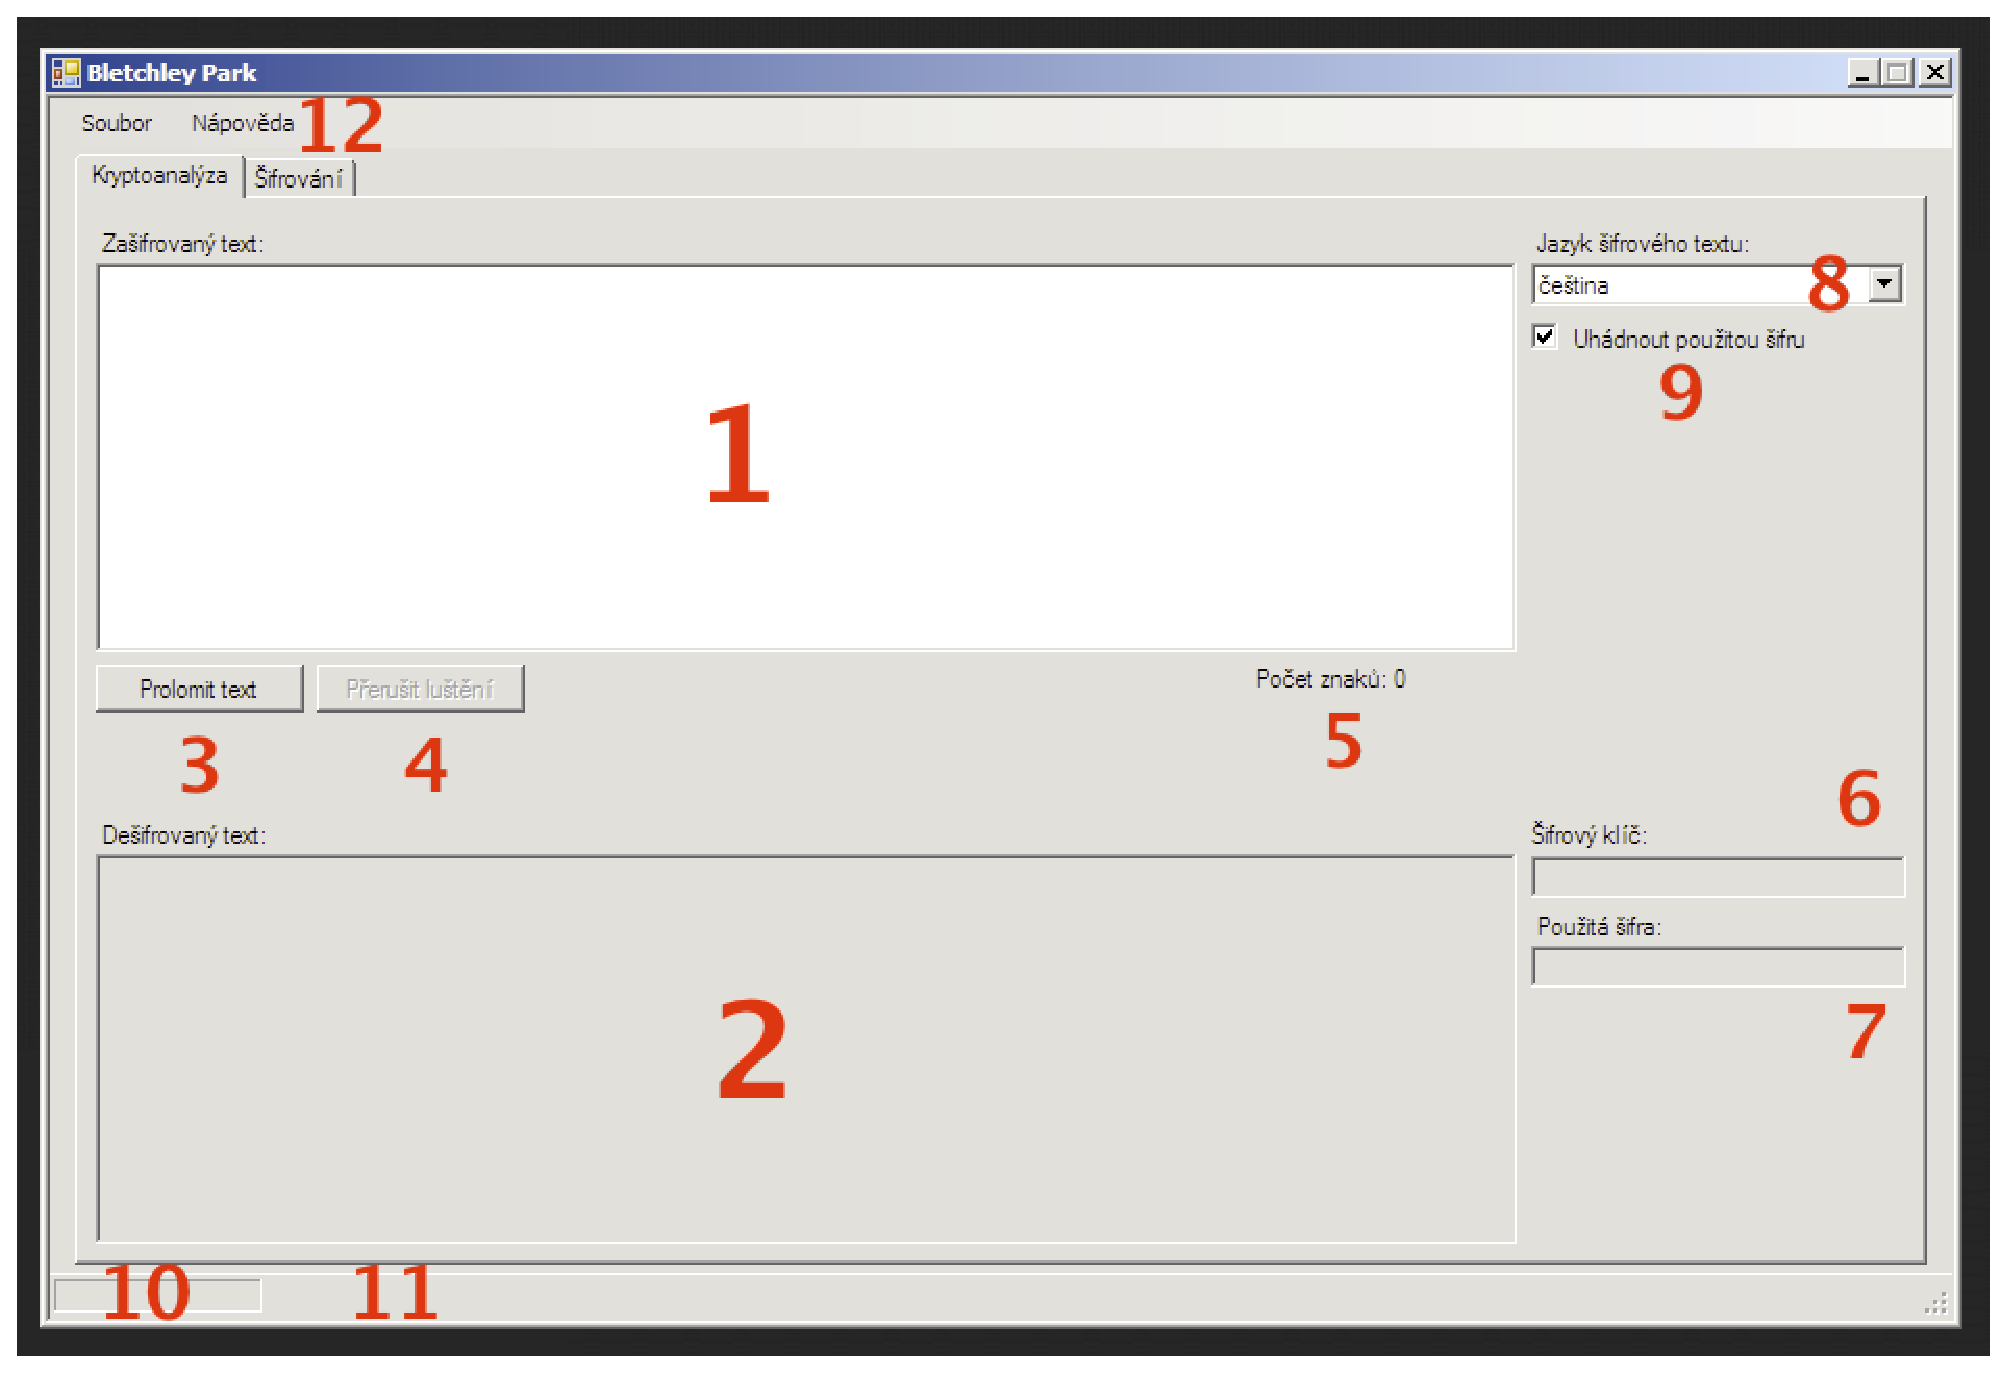
\includegraphics[scale=0.4]{images/cryptauto.eps}
  \end{center}
\caption{Kryptoanalytická část aplikace}
\label{img_crypt}
\end{figure}

Popis všech ovládacích prvků:

\begin{enumerate}
\item Primární textové pole, do kterého uživatel vkládá text, který chce rozluštit. Textové pole podporuje kontextové menu, které umožňuje jednoduše smazat celý text a vložit na místo něj text ze schránky a případně i nakopírovat celý text do schránky.
\item Sekundární textové pole, které zobrazuje výsledek luštění. V~případě úspěšného prolomení šifry se zde objeví dešifrovaný text. Nepodaří-li se text prolomit, zobrazí se zde upozornění. Pole podporuje kontextové menu, které umožňuje jednoduše nakopírovat celý text do schránky. 
\item \label{startattack} Tlačítko, které spouští luštění. Během samotného luštění je neaktivní. 
\item Tlačítko, kterým může uživatel v~případě potřeby přerušit luštění. Je aktivní pouze během aktivního luštění. 
\item Ukazatel počtu napsaných znaků v~primárním textovém poli. 
\item Textové pole, které na konci úspěšného luštění zobrazí uhádnutý šifrovací klíč. 
\item Textové pole, které na konci úspěšného luštění zobrazí použitou šifru.
\item \label{langchoise} Rozbalovací menu, které obsahuje několik jazyků a umožňuje uživateli nastavit, v jakém jazyce je vložený šifrový text (podporovány jsou tyto jazyky: čeština, angličtina, němčina a francouzština). Bez správného určení jazyka se algoritmy nebudou chovat správně. 
\item \label{autocheck} Checkbox, který indikuje, zda má aplikace sama určit použitou šifru (při zapnutém checkboxu) nebo zda uživatel sám zvolí, jakou šifrou byl text zašifrován.
\item \label{progressbar} Progress bar, který při startu aplikace indikuje průběh načítání slovníků, později zobrazuje průběh kryptoanalýzy.
\item \label{statusbar} Status bar -- aplikace zde po najetí kurzorem na nějaký ovládací prvek zobrazuje pomocné informace.
\item \label{hlavnimenu} Hlavní menu aplikace, obsahuje základní funkce programu a nápovědu. 
\end{enumerate}

V~případě, že pomocí checkboxu zvolíme režim, kdy si uživatel může sám vybrat použitou šifru (viz ovládací prvek \ref{autocheck} na obrázku \ref{img_crypt}), získáme další možnosti nastavení, viz obrázek \ref{img_usercheck}

\begin{figure}[h]
  \begin{center}
  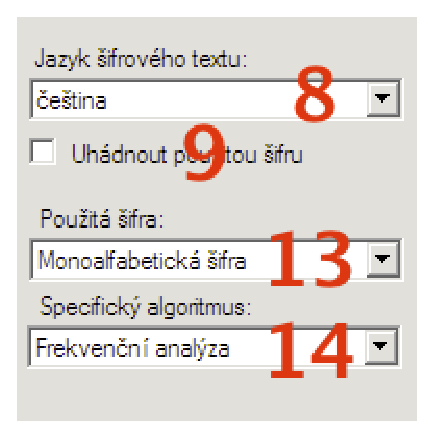
\includegraphics[scale=0.8]{images/cryptchoise.eps}
  \end{center}
\caption{Možnosti voleb uživatele, pokud vypne automatické zjišťování použité šifry}
\label{img_usercheck}
\end{figure}

Popis nových voleb:

\begin{enumerate}
\setcounter{enumi}{12}
\item Výběr šifry, kterou je zašifrován šifrový text, tj. text vložený v~primárním textovém okně. 
\item Výběr algoritmu, který bude použit při luštění. Některé šifry nabízí více různých algoritmů, které mohou pro stejný text vrátit jiné výsledky. V~případě, že jeden algoritmus nedokáže šifru vyluštit, může uživatel zkusit jiný algoritmus.
\end{enumerate}

\subsubsection{Typický příklad užití kryptoanalytické záložky}
Záložka a všechny její ovládací prvky jsou uzpůsobeny k~co možná nejjednodušší práci s~algoritmy luštící šifry. 

Na začátku máme nějakou zašifrovanou zprávu a chceme získat původní otevřený text. Spustíme aplikaci a nakopírujeme tento text do primárního textového pole. Pokud byl původní text jiného jazyka než českého, zvolíme ještě v~comboboxu požadovaný jazyk (ovládací prvek \ref{langchoise}). Dále klikneme na tlačítko \uv{Prolomit text} (ovládací prvek \ref{startattack}). Aplikace bude chvíli počítat a po několika sekundách se objeví výsledek -- buď správně či nesprávně vyluštěný text nebo upozornění, že text nebylo možné rozluštit. 

Známe-li šifru, kterou byl náš šifrový text zašifrován, můžeme odškrtnout \uv{Uhádnout použitou šifru} (ovládací prvek \ref{autocheck}) a specifikovat, kterou šifrou byl text zašifrován. Poté opět stiskneme tlačítko \uv{Prolomit text} (ovládací prvek \ref{startattack}). Doba luštění bude kratší, aplikace nebude muset zkoušet všechny šifry. 

Obecně platí, že čím delší text, tím větší je pravděpodobnost, že bude správně rozluštěn. U~Caesarovy šifry stačí text dlouhý řádově stovky znaků, ostatní šifry už jsou složitější a vyžadují řádově tisíce znaků. 

Některé algoritmy mají kvůli efektivitě a rychlosti nastavenou maximální délku klíče, kterou jsou schopny vyluštit. Algoritmy u Caesarovy šifry a monoalfabetické substituční šifry pracují bez omezení, algoritmus u Jednoduché sloupcové transpozice (\ref{testkeylengthtransattack}) má maximální délku klíče nastavenou na 12, algoritmus Hrubé síly (\ref{brutevig}) u Vigenèrovy šifry má maximální délku klíče 20 a algoritmus Odhadnutím délky klíče (\ref{testkeylengthvig}) má maximální délku 40. Aplikace neobsahuje algoritmus pro prolomení monoalfabetické šifry bez ponechaných mezer, takový šifrový text aplikace nedokáže prolomit. 

\subsection{Šifrovací část}
\subsubsection{Popis jednotlivých ovládacích prvků}
Šifrovací část se nachází na záložce \uv{Šifrování} a slouží k~šifrování a dešifrování zpráv, pokud předem známe šifrovací klíč. Šifrovací záložka je vidět na obrázku\,\ref{img_encrypt} 

\begin{figure}[h]
  \begin{center}
  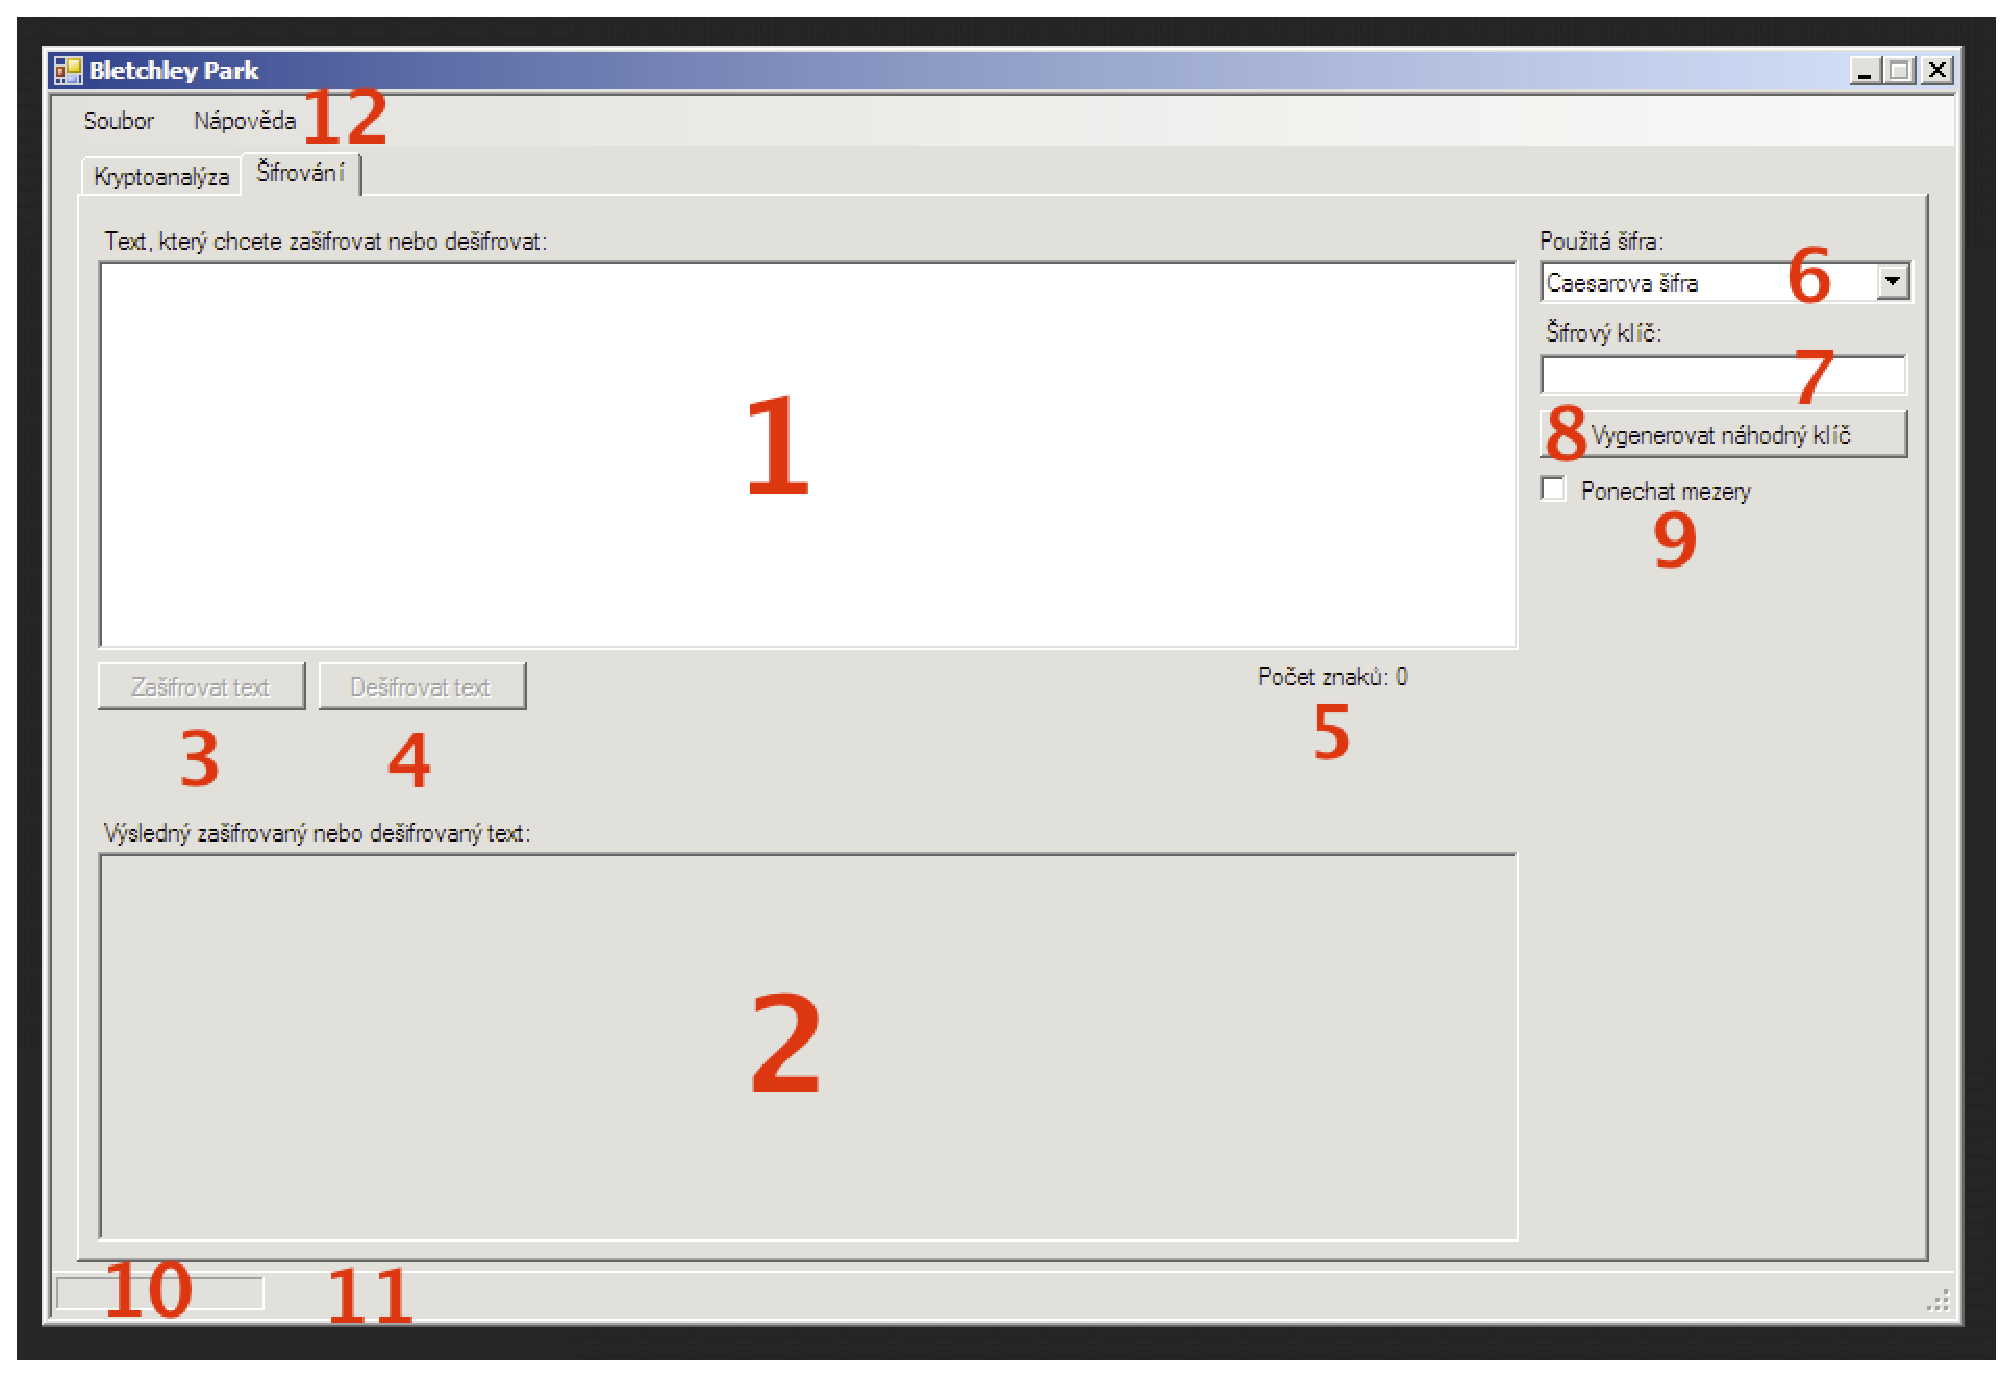
\includegraphics[scale=0.4]{images/encrypt.eps}
  \end{center}
\caption{Šifrovací část aplikace}
\label{img_encrypt}
\end{figure}

%antisux
\newpage
Popis ovládacích prvků:

\begin{enumerate}
\item Primární textové pole. Zde uživatel vkládá text, který chce šifrovat nebo dešifrovat. Textové pole podporuje kontextové menu, které umožňuje jednoduše smazat celý text a vložit na místo něj text ze schránky a případně i nakopírovat celý text do schránky.
\item Sekundární textové pole. V~tomto textovém poli se zobrazí výsledný šifrový nebo otevřený text. I~toto pole podporuje kontextové menu pro snadné nakopírování obsahu do schránky. 
\item \label{encryptbutton} Stisknutím tohoto tlačítka aplikace zašifruje text z~primárního textového pole a výsledek zobrazí v~sekundárním poli.
\item \label{decryptbutton} Stisknutím tohoto tlačítka aplikace dešifruje text z~primárního textového pole a výsledek zobrazí v~sekundárním poli. 
\item Zobrazuje počet znaků napsaných v~primárním poli. 
\item \label{ciphers} Combobox, který nabízí různé druhy šifrových algoritmů. Touto volbou uživatel specifikuje, jakou šifrou si přeje text šifrovat nebo dešifrovat. 
\item \label{cipherkey} Textové pole, kam uživatel vepíše použitý šifrovací klíč. 
\item \label{randomkey} Tlačítko, kterým může uživatel vygenerovat náhodný klíč, nechce-li použít žádný vlastní. Vždy vygeneruje validní klíč pro zvolenou šifru. Pokud je textové pole podbarvené zeleně, je vepsaný klíč validní. Pokud je podbarvené červeně, není validní. Informace o~tom, jaká pravidla musí klíč splňovat se nachází ve status baru. 
\item Checkbox indikuje, jestli má aplikace při šifrování ponechat v~šifrovém textu mezery, které budou reprezentovat hranice mezi slovy. Aplikace ponechá vždy jen jednu mezeru, všechny ostatní bílé znaky budou ignorovány. Jakékoliv další formátování (tabulátory, odřádkování apod.) bude ignorováno.  
\item Progress bar, který zobrazuje průběh šifrování a dešifrování. Obvykle jen problikne, protože šifrování i dešifrování je rychlé. 
\item Status bar -- aplikace zde po najetí kurzorem na nějaký ovládací prvek zobrazuje pomocné informace, po aktivaci textového pole pro zadání klíče \ovl{cipherkey} se zde například zobrazují podrobnosti o~tom, jak má vypadat šifrovací klíč. 
\item Hlavní menu aplikace, obsahuje základní funkce programu a nápovědu. 
\end{enumerate}

\subsubsection{Typický příklad použití šifrovací záložky}
Uživatel může v~této záložce provádět dvě opačné úlohy: může šifrovat text a dešifrovat text. 

Pokud si přeje šifrovat text, vloží svou zprávu, kterou chce zašifrovat, do primárního textového pole. Následně si vybere šifru, kterou chce text zašifrovat \ovl{ciphers} a do textového pole \ovl{cipherkey} vepíše šifrovací klíč, který chce použít. Pokud nechce použít konkrétní šifrovací klíč, může si nechat vygenerovat náhodný klíč (ovládací prvek \ref{randomkey}). Nakonec stiskne tlačítko \uv{zašifrovat text} \ovl{encryptbutton}. V~sekundárním textovém poli se zobrazí výsledný šifrový text. Vyvoláním kontextového menu lze šifrový text jednoduše nakopírovat do schránky. 

Přeje-li si uživatel naopak dešifrovat text, vloží svůj zašifrovaný text do primárního textového pole, vybere si šifru, kterou byl text zašifrován \ovl{ciphers} a do textového pole \ovl{cipherkey} vepíše šifrovací klíč. Nakonec stiskne tlačítko \uv{dešifrovat text} \ovl{decryptbutton} a v~sekundárním textovém poli se zobrazí původní otevřený text.



%%%%%%%%%%%%%%%%%%%%%%%%%%%%%%%%%%%%%%%%%%%%%%%%%%%%%%%%%%%%%%
%%%%%%%%%%%%%%%%%%%%%%%%%%%%%%%%%%%%%%%%%%%%%%%%%%%%%%%%%%%%%%
%%%%%%%%%%%%%%%%%%%%%%%%% DOKUMENTACE %%%%%%%%%%%%%%%%%%%%%%%%%
%%%%%%%%%%%%%%%%%%%%%%%%%%%%%%%%%%%%%%%%%%%%%%%%%%%%%%%%%%%%%%
%%%%%%%%%%%%%%%%%%%%%%%%%%%%%%%%%%%%%%%%%%%%%%%%%%%%%%%%%%%%%%
\newpage
\section{Dokumentace zdrojového kódu}
Aplikace je napsána v~programovacím jazyku C\# a běží na .NET frameworku. Je rozdělena do tří oddělených částí: GUI aplikace, DLL knihovna \code{CryptanalysisCore} obstarávající všechny šifrovací algoritmy a DLL knihovna \code{ExtensionMethods}.


\subsection{CryptanalysisCore}
\label{cryptocore}

Obsahuje všechny algoritmy vztahující se k~šifrování, dešifrování a luštění šifer. Knihovna je rozdělena do několika dalších částí:

\subsubsection{Ciphers}
Tato část obsahuje třídy, které přímo reprezentují jednotlivé šifry. Hlavní třídou je třída \code{Cipher}, ze které ostatní třídy dědí. Tato třída obsahuje základní metody pro šifrování, dešifrování, luštění šifer, generování náhodného klíče a pro kontrolu, zda je klíč validní. Potomci třídy si tyto metody přepisují po svém. Dále obsahuje pole delegátů \code{CrackMethods}, ve kterém jsou uloženy reference na implementované kryptoanalytické algoritmy. Toto pole naplňují až konkrétní šifry metodou \code{SetCrackMethods} podle toho, jaké algoritmy implementují. 

Ostatní třídy jsou: \code{Caesar}, \code{Monoalphabetic}, \code{Transposition} a \code{Vigenere} a reprezentují konkrétní šifru. Každá z~těchto tříd obsahuje vlastní kryptoanalytické algoritmy, které často využívají struktury a třídy z~dalších částí knihovny. 
 
Nejdůležitější metodou je zde metoda \code{Crack}, která bere na vstupu šifrový text, číselný identifikátor konkrétního algoritmu a identifikátor jazyka. Na výstupu vrací vyluštěný klíč, v~případě neúspěchu vyvolá výjimku \code{MatchNotFound} (viz \ref{exceptions}).
 
 \subsubsection{Exceptions}
 \label{exceptions}
 Obsahuje výjimky, se kterými aplikace pracuje. 
 
 \begin{description}
  \item[\code{InvalidCipherKey}] oznamuje neplatný šifrový klíč pro danou šifru.
  \item[\code{InvalidOpentext}] oznamuje neplatný otevřený text.
  \item[\code{InvalidCiphertext}] oznamuje neplatný šifrový text.
  \item[\code{MatchNotFound}] kryptoanalytický algoritmus nenalezl žádný shodný klíč. 
\end{description}

\subsubsection{Filters}

Tato část obsahuje pomocné algoritmy ve formě tříd, které umožňují lepší rozdělení odpovědnosti. Jsou zde funkce využívané obvykle při kryptoanalýze, například různé filtrování slov na základě slovníkového útoku, algoritmus pro zjištění možných délek klíče u~Vigenèrovy šifry apod. 

\subsubsection{HelpMethods}

Obsahuje obecné pomocné metody pro práci s~textem, dodatečné matematické metody jako například zjištění všech dělitelů čísla, kombinatorické metody pro zjištění permutací, variací apod. Velká část metod je natolik obecná, že jdou použít i mimo tento program. 

\subsubsection{Structures}

Obsahuje pomocné struktury pro některé algoritmy. Obsahuje ale i dvě důležité struktury:

\begin{description}
\item[\code{LangCharacteristic}] Struktura obsahující statistické informace o~daném jazyku. Uchovává informace o~frekvenci písmen, bigramů, trigramů, slovník všech a slovník nejčastějších slov a další potřebné informace. 
\item[\code{Storage}] Nejdůležitější struktura, obsahuje pole struktur \code{LangCharacteristic} pro každý podporovaný jazyk, dále uchovává seznam šifer, které můžeme použít a seznam jazyků. Stará se také o~samotné načítání těchto informací pomocí metody \code{LoadFiles}. Aplikace po zavolání této metody načte potřebné slovníky a další informace ze složky, jejíž jméno je uloženo ve statické proměnné \code{StatsFolderName}. Proměnná je \code{public}, takže ji lze měnit hodnotu ještě před zavoláním metody \code{LoadFiles}. V~proměnné \code{StatsFolderPath} je pak uložena celá cesta ke slovníkům. Pomocí metody \code{GetLangChar} lze získat statistiky konkrétního jazyka.
\end{description}


\subsection{GUI aplikace}
Tato část obsahuje metody pro vykreslení a ovládání GUI celé aplikace. Zároveň se stará o~správné volání kryptoanalytických metod, které volá z~knihovny popsané v~kapitole \ref{cryptocore} I~tato část je rozdělena do dalších podčástí:

\subsubsection{Window}
Obsahuje samotné metody pro obsluhu událostí. Tyto metody typicky nevykonávají funkční kód přímo, ale volají nějakou další obslužnou metodu.

\subsubsection{Window\_Properties}
Obsahuje vlastnosti definované celému oknu. Jsou zde abstrakční bariéry pro nastavování hodnot do textových polí nebo nastavování stavu \code{Enabled} checkboxům a položkám v~menu apod. Vlastnosti slouží především k~větší přehlednosti. Pro každou šifru uchovává objekt vytvořený z~požadované třídy. Při šifrování, dešifrování nebo luštění se pouze vybere aktuální šifra a zavolá se jedna z~obslužných metod.

\subsubsection{Window\_Functions}
Obsahuje funkční metody, které jsou volány z~\code{Window}. Pokud uživatel klikne na nějaké tlačítko, v~části \code{Window} se nachází kód k~odchycení této události a tento kód následně zavolá nějakou funkci z~\code{Window\_Functions}, která obslouží zbytek požadavku. Výhoda spočívá v~tom, že pokud dva ovládací prvky mají udělat totéž (například tlačítko a položka v~menu), nemusí se žádný kód opakovat, jen se zavolá stejná funkce z~\code{Window\_Functions}.

\subsubsection{Window\_Statutes}
Obsahuje metody, které mají za úkol měnit text ve status baru podle aktuálního stavu v~aplikaci. 



\subsection{ExtensionMethods}
Další DLL knihovna, která obsahuje obecné Extension Methods, které rozšiřují schopnosti vestavěných tříd. Je to knihovna zcela nezávislá na zbytku a lze ji připojit k~jakémukoliv jinému projektu. Rozšiřuje například \code{int} o~metodu \code{times}, která bere jako parametr metodu, která se provede tolikrát, kolik je hodnota \code{int}u, se kterým metodu voláme. Dalším příkladem je metoda \code{RemoveDiacritics} připojená ke \code{string}u, která odstraňuje diakritiku z~řetězce. 









%%%%%%%%%%%%%%%%%%%%%%%%%%%%%%%%%%%%%%%%%%%%%%%%%%%%%%%%%
%%%%%%%%%%%%%%%%%%%%%%%%%%%%%%%%%%%%%%%%%%%%%%%%%%%%%%%%%%
%%%%%%%%%%%%%%%%%%%%%%%%% DODATKY %%%%%%%%%%%%%%%%%%%%%%%%%
%%%%%%%%%%%%%%%%%%%%%%%%%%%%%%%%%%%%%%%%%%%%%%%%%%%%%%%%%
%%%%%%%%%%%%%%%%%%%%%%%%%%%%%%%%%%%%%%%%%%%%%%%%%%%%%%%%%
\newpage
\section{Dodatky}
\subsection{Statistické informace $\stats$}
\label{stats}
Kryptoanalytické algoritmy popsané v~kapitole \ref{crypto_chapter} potřebují znát specifické statistické údaje o~jazyku, nad kterým zrovna pracují. Tato sada informací se skládá z~těchto částí: 

\begin{itemize}
\item procentuální vyjádření výskytu jednotlivých znaků, bigramů a trigramů v~daném jazyku,
\item procentuální vyjádření výskytu jednotlivých písmen na začátku a na konci slov,
\item průměrný počet různých písmen vyskytující se za daným písmenem v~textu o~přiměřeně dlouhé délce (zvolil jsem tisíc znaků),
\item seznam \uv{všech} slov daného jazyka,
\item seznam nejčastějších slov jazyka.
\end{itemize}

Tyto informace jsem pro každý jazyk zvlášť získal analýzou dlouhého textu v~daném jazyce. Do tohoto textu jsem vždy zahrnul několik tisíc článků stažených z~internetu a případně i několik knih v~elektronické podobě, které jsou volně k~dostání. Dále jsem použil slovníky pro kontrolu překlepů pro textový editor PSPad, ke stažení na adrese \texttt{<http://www.pspad.com/cz/download.php>}.

\subsection{Metodika měření úspěšnosti algoritmů}
\label{metodika}
Pro testování jsem použil text (označme $t$), ze kterého jsem generoval statistické informace $\stats$, viz \ref{stats} Postup byl pro každý algoritmus následující:

\begin{enumerate}
\item Vygenerujeme náhodný validní klíč $K_o$ pro danou šifru.
\item Z~textu $t$ vybereme řetězec $O$ dlouhý $n$ znaků -- podle toho, jak dlouhý text chceme zkoušet vyluštit (v~tabulkách v~kapitole \ref{crypto_chapter} to odpovídá hodnotám ve sloupci \uv{počet znaků}).
\item Zašifrujeme text $O$ pomocí klíče $K_o$. Vznikne šifrový text $C$.
\item pomocí daného algoritmu zkusíme vyluštit šifrový text $C$. Algoritmus buď selže nebo vrátí nějaký klíč $K_c$.
\end{enumerate}

V~tuto chvíli porovnáme klíče $K_o$ a $K_c$. Každá šifra má svou specifickou funkci (viz dále), která určí, zda bychom s~klíčem $K_c$ úspěšně dešifrovali otevřený text $O$. Nakonec spočítáme počet úspěšně vyluštěných textů děleno počtem všech testovaných textů a máme poměr vyjadřující úspěšnost algoritmu. Všechny algoritmy jsem nechal vyluštit tisíc textů. Výsledek jsem zaokrouhloval na jednotky procent.

Každá šifra má jinou funkci, která rozhoduje, zda bychom s~klíčem správně dešifrovali šifrový text. Klíče $K_o$ a $K_c$ nemusí vždy shodovat, aby byl výsledný dešifrovaný text čitelný. Definujeme tato pravidla:

 \begin{itemize}
\item Pokud pracujeme s~Caesarovou šifrou, musí být klíče $K_o$ a $K_c$ shodné. 
\item Pokud pracujeme s~monoalfabetickou šifrou, může klíč $K_c$ obsahovat celkem šest různých chybných substitucí. Buď zcela nevyluštěných (typicky pro písmena \uv{x}, \uv{w} nebo \uv{q}, které se v~českém textu vyskytují sporadicky) nebo chybných substitucí. I~při šesti chybách zůstává text obvykle bez větších problémů čitelný. 
\item Pokud pracujeme s~Vigenèrovou šifrou, může klíč $K_c$ obsahovat jedno chybné písmeno. Pokud máme například klíč o~délce šest, pak na jedno špatně dešifrované písmeno připadá pět správně dešifrovaných písmen. Text bude i tak bez větších problémů čitelný. Čím delší klíč, tím čitelnější text bude.
\item Pokud pracujeme s~transpoziční šifrou, musí být klíče $K_o$ a $K_c$ shodné. 
\end{itemize}

Úspěšnost jsem měřil pouze pro české texty. Výsledky jsou pouze orientační, slouží především k bližší představě o tom, jak dlouhý by měl být vstupní šifrový text.

\subsection{Obsah přiloženého CD}

Popis jednotlivých složek na přiloženém CD: 

\begin{description}
\item[\texttt{bin/}] Složka obsahující zkompilované soubory určené k běhu aplikace bez nutnosti instalace. Spouštěcí soubor se jmenuje \texttt{BletchleyPark.exe}. V dalších podsložkách se nachází nápověda a pomocné statistické informace o jazycích. 

\item[\texttt{src/}] Složka obsahující zdrojové soubory potřebné k sestavení celé aplikace. Aplikaci jsem vytvářel ve vývojovém prostředí {\em Microsoft Visual Studio 2008}.%, v jiné verzi jsem sestavování netestoval.

\item[\texttt{doc/}] Složka obsahující text bakalářské práce ve formátu PDF včetně zdrojových souborů v \LaTeX u a obrázků ve formátu EPS i PNG. 

\item[\texttt{readme.txt}] Textový soubor obsahující základní pokyny a popis struktury CD. 
\end{description}










\begin{conclusions-cz}
Podařilo se mi naprogramovat aplikaci, která zvládá na běžném počítači luštit v~řádu sekund celkem čtyři různé druhy šifer. Úspěšnost algoritmů je uspokojující pro delší texty, výsledky pro kratší texty jsou horší a existuje zde prostor pro vylepšení. Aplikace umí luštit šifrový text v~celkem čtyřech různých jazycích -- v~češtině, angličtině, němčině a francouzštině. Pro každý jazyk se používá stejný kryptoanalytický algoritmus, pouze s~jinými statistickými informacemi o~daném jazyku -- proto je možné přidat do aplikace podporu pro další jazyk.

Všechny použité algoritmy jsou důsledně sepsány a specifikovány, včetně několika nápadů na jejich vylepšení či změnu. U~každé použité šifry jsem zmínil i její nevýhody, na kterých jsem následně stavěl kryptoanalýzu. Ne všechny nevýhody ale byly využity, takže v~případě dalšího vývoje aplikace může cesta pokračovat buď vylepšením stávajících algoritmů nebo se mohou využít právě tyto nepoužité nevýhody.
\end{conclusions-cz}
















\newpage
\bibliographystyle{czechiso}
%\bibliographystyle{alpha}
\bibliography{bakalarka}

\end{document}